\documentclass[11pt,a4paper]{article}
\usepackage[margin=2.2cm]{geometry}
\usepackage[T1]{fontenc}
\usepackage[utf8]{inputenc}
\usepackage{lmodern}
\usepackage{graphicx}
\usepackage{booktabs}
\usepackage{longtable}
\usepackage{array}
\usepackage{enumitem}
\usepackage{hyperref}
\usepackage{xcolor}
\hypersetup{colorlinks=true, linkcolor=blue!50!black, urlcolor=blue!50!black}
\graphicspath{{figures/}}
\setlength{\parskip}{4pt}
\title{ProGenome: a federated workflow for genome-graph and proteomic integration\\[6pt]\large Complete knowledge-transfer document: problem, biology, data, pipeline, knowledge graph, models, federated learning, deployment and results}
\author{Team \#3, Nordic Biobank x NVIDIA Federated Learning Hackathon, Copenhagen, September 2026. Branch: modelling. Author of this build: Koushik Telaprolu (genomics/ pipeline), with the team's proteomics and README work referenced where used.}
\date{18 September 2026}
\begin{document}
\maketitle
\tableofcontents
\newpage

\section{How to read this document}

This is written for a teammate who joins today and knows nothing about the biology, the software, the models or the infrastructure. Part I is a primer that defines every concept used later. Part II is the whole workflow on a few pages: what goes in and what comes out of every stage, where each data source is used, what the trained model produces and how it is used, ground truth against prediction, where the language model sits, and how every item of the team README on branch main is covered. Part III is the project in depth, in the order the data flows: problem, data sources, data pipeline, exploratory analysis, knowledge graph, embeddings, the graph neural network (the encoder), the language-model decoder, the federated training, deployment, results and caveats. Part IV is how to run everything, a glossary and a repository map. Every number is measured on chromosome 22 with random seed 42 and comes from files under genomics/outputs; nothing is typed in from memory.

\section{Part I: Primer}

\subsection{Biology in ten minutes}

DNA is a long text written in four letters (A, C, G, T). Humans have about 3 billion letters, packaged in 23 pairs of chromosomes; chromosome 22 is one of the smallest, about 50 million letters. Everyone carries two copies of each chromosome, one from each parent. A gene is a region of DNA that encodes a protein; proteins are the molecules that do the work in cells, and measuring how much of each protein a person has is called proteomics.

Two people's DNA differs at roughly one letter in a thousand; those positions are variants. A haplotype is the specific combination of variants along one copy of a chromosome. Because DNA is inherited in chunks (recombination cuts and rejoins the parental copies at a limited number of places), neighbouring variants tend to travel together. A haploblock is a stretch of chromosome between recombination hotspots that is usually inherited as one unit. Phased data means we know, for every variant, which of the two copies it sits on, so each person's two haplotypes per block are known separately.

The 1000 Genomes Project (1000G) sequenced 2,548 people from 26 populations grouped into five continental ancestries: AFR (African), AMR (admixed American), EAS (East Asian), EUR (European) and SAS (South Asian). It recorded only ancestry, population and sex about them, nothing clinical. A phenotype is any observable property of a person; in this project the real phenotypes are those three, and a clinical-looking case/control phenotype had to be simulated.

\subsection{Software in ten minutes}

Python is the language of every script here; pandas handles tables, scipy handles sparse matrices (mostly-zero grids stored compactly), PyTorch does neural networks and PyTorch Geometric (PyG) adds graph neural networks. Git tracks versions of the code; a branch is a parallel line of work (ours is called modelling). Docker packages the code and every library it needs into an image so it runs identically on any machine. A GPU is a processor built for many small parallel calculations; CUDA is NVIDIA's software that lets PyTorch use it. NVIDIA Brev rents GPU machines by the hour. Neo4j is a database made for graphs, with a browser to look at them.

\subsection{Data science in ten minutes}

Exploratory data analysis (EDA) means measuring and plotting the data before modelling: sizes, distributions, missing values, obvious structure. To judge a model honestly the people are split once into train (learn), validation (choose settings and when to stop) and test (report only once, at the end); here 70/15/15 percent, chosen at random but stratified so each ancestry is represented in every part. Accuracy is the fraction correct; balanced accuracy averages the accuracy per class so a rare class cannot be ignored; AUC (area under the ROC curve) is the probability that a random case is scored higher than a random control, 0.5 is guessing and 1.0 is perfect. A negative control is a target that must come out at chance level if the method is sound.

\subsection{Machine learning in ten minutes}

An embedding is a list of numbers (a vector) that represents an object so that similar objects get similar vectors. A graph is a set of nodes joined by edges; a knowledge graph is a graph whose nodes and edges have types and properties. A graph neural network (GNN) computes a vector for every node by repeatedly mixing each node's own vector with those of its neighbours (message passing); after two rounds a node's vector summarises its two-hop neighbourhood. Training means adjusting the network's weights so that a prediction made from those vectors matches known labels, measured by a loss; an optimiser (Adam) nudges the weights to reduce the loss, one epoch being one pass over the data. An encoder turns raw data into vectors; a decoder turns vectors (and retrieved facts) into an output, here text written by a large language model (LLM). Retrieval-augmented generation (RAG) gives the LLM the facts it should use so it does not invent them; GraphRAG retrieves those facts from a graph.

\subsection{Federated learning in five minutes}

Hospitals cannot pool patient data. Federated learning trains one model across sites without moving records: each site trains the shared model on its own data for a few steps, sends only the updated weights to a coordinator, the coordinator averages them (FedAvg) and sends the average back; repeat for several rounds. NVIDIA FLARE (NVFlare) is the framework that runs this loop; its simulator runs all sites on one machine so the workflow can be tested before real deployment.

\section{Part II: The workflow on a few pages}

\subsection{The story, stage by stage}

Read the workflow as one sentence first: a public graph of haplotype clusters is joined to people by their sample id; each person's row of that graph, their phenotype labels and their protein measurements are attached to a person node; a graph neural network is trained to predict a label from the person's neighbourhood; the trained network yields predictions, an embedding per person and cluster, a saliency per cluster and a set of weights; the predictions and embeddings are checked against ground truth, a language model turns them into a cited report per person, and the weights are what a federated deployment exchanges instead of data. Every stage below is one script with one Makefile target.

\begin{figure}[htbp]
\centering
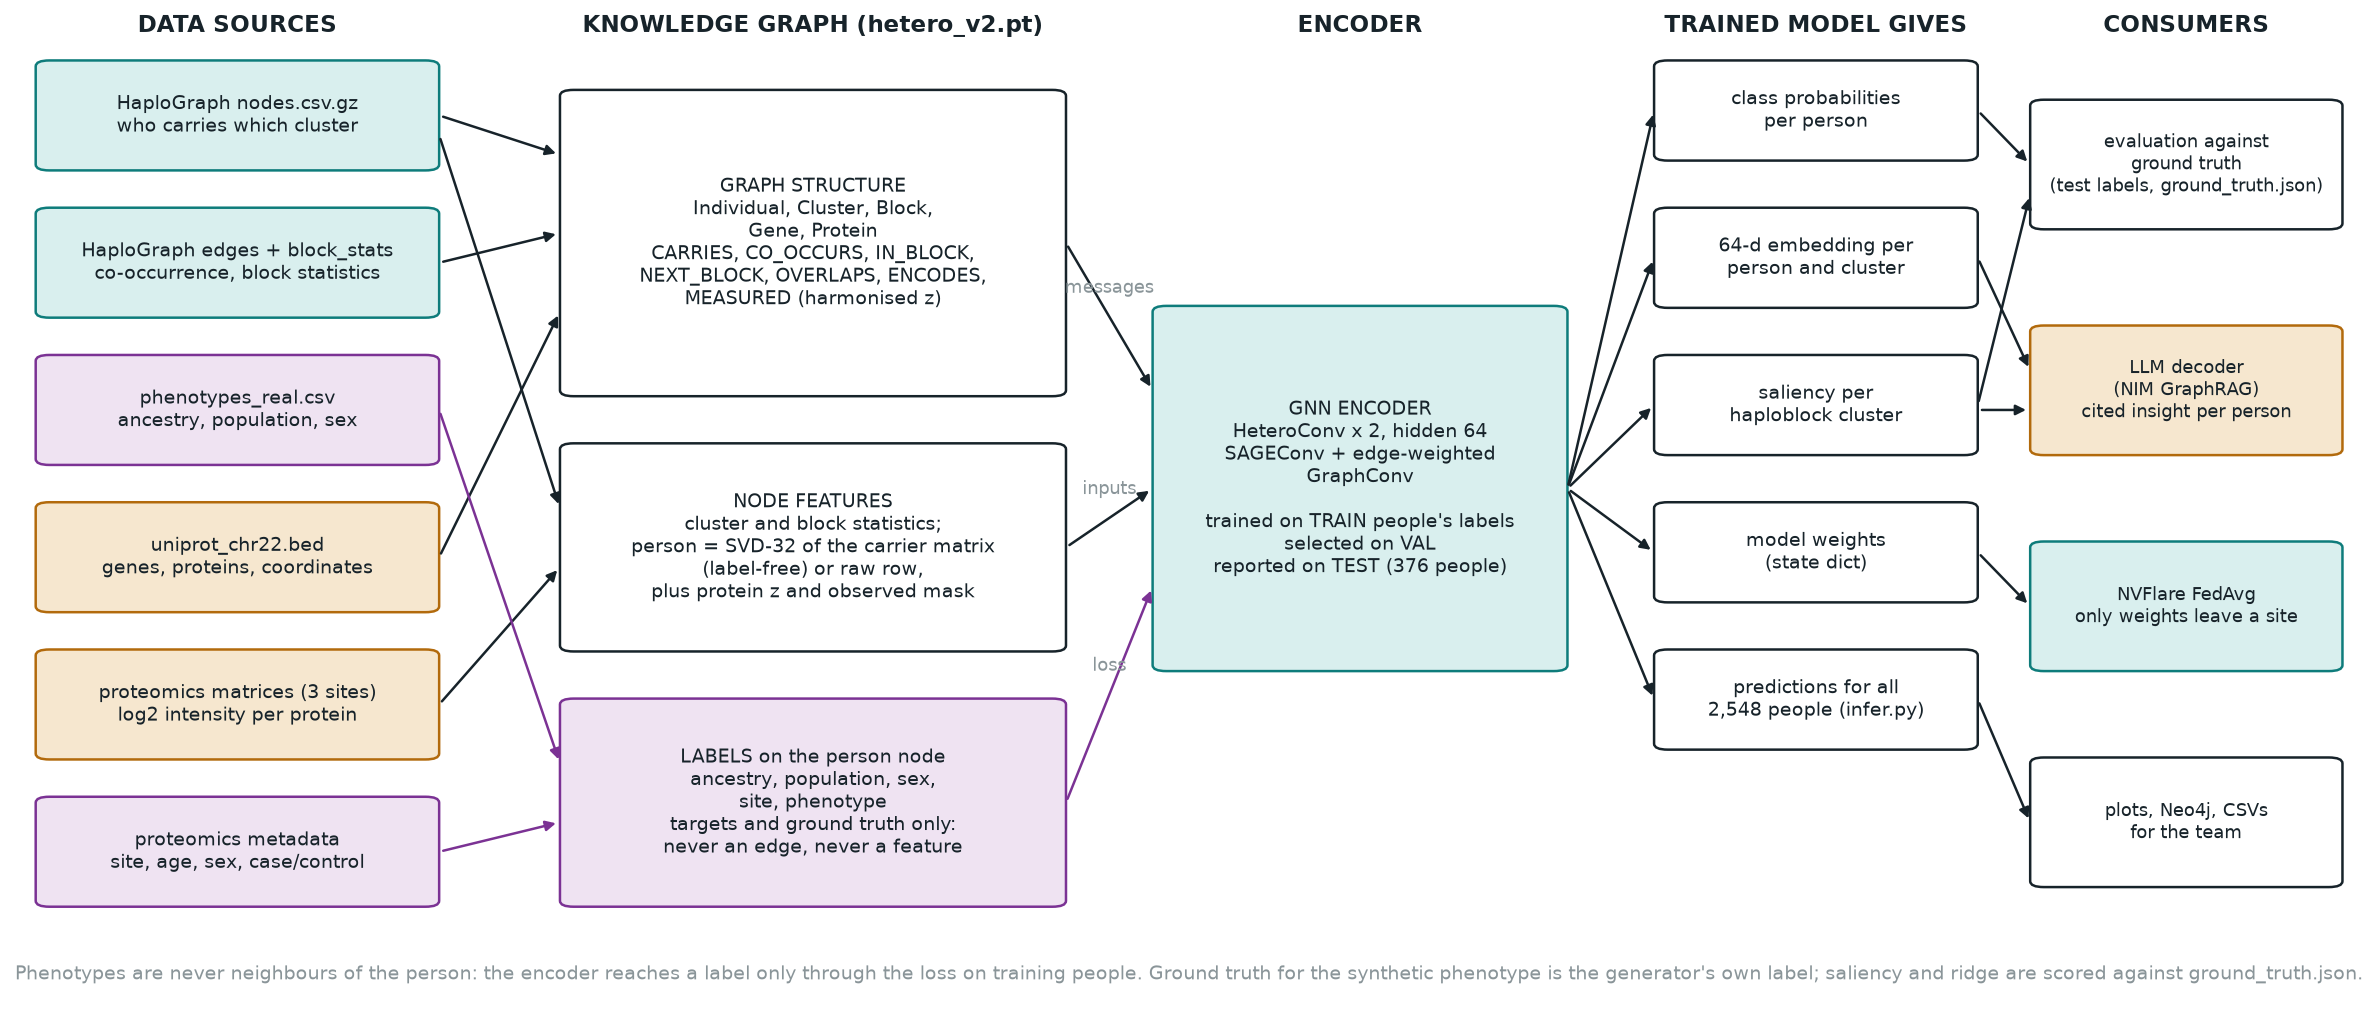
\includegraphics[width=0.98\linewidth]{data_flow_map.png}
\caption{Where each data source enters, what the trained model produces, and where each product goes.}
\end{figure}

\begin{longtable}{p{0.132\linewidth}p{0.282\linewidth}p{0.357\linewidth}p{0.169\linewidth}}
\toprule
\textbf{Stage} & \textbf{What goes in} & \textbf{What comes out} & \textbf{Lands in} \\
\midrule
\endhead
1 download & URLs on data.haploblocks.org & HaploGraph node and edge files, phenotypes, block statistics, md5-verified & data/ \\
2 knowledge graph v1 & nodes.csv.gz (who carries which cluster), edges (which clusters co-occur), block statistics, phenotypes & Individual, Cluster, Block nodes; CARRIES, CO\_OCCURS, IN\_BLOCK, NEXT\_BLOCK edges; labels stored on the person nodes & outputs/kg/chr22/ (carries.npz, hetero.pt) \\
3 statistics & the graph and the labels & for every cluster and edge, how strongly it tracks ancestry, population and sex (Cramer's V, FDR) & outputs/cooccurrence/chr22/ \\
4 baseline and split & carrier matrix and labels & logistic-regression scores to beat; the single train/val/test split every later model reuses & outputs/baseline/, outputs/splits/ \\
5 starting embeddings & carrier matrix only, no labels & a 32-number vector per person and per cluster (SVD), or Node2Vec, learned, or the raw row & computed inside training \\
6 GNN v1 (encoder) & graph, starting vectors, and the labels of training people only & trained weights; class probabilities per person; a 64-number embedding per person and per cluster & outputs/gnn/chr22/<target>\_<init>/ \\
7 embedding check & SVD and GNN embeddings, labels of test people & silhouette and nearest-neighbour accuracy, 2-D plots & outputs/embeddings/chr22/ \\
v2.1 synthetic proteomics & the real 1000G ids, the carrier matrix, the gene BED & 3 per-site protein matrices, metadata (site, age, sex, case/control), ground\_truth.json & outputs/proteomics\_synth/chr22/ \\
v2.2 knowledge graph v2 & graph v1, gene BED, proteomics & Gene and Protein nodes; OVERLAPS, ENCODES, MEASURED edges (harmonised z); site and phenotype labels on people & outputs/kg/chr22/hetero\_v2.pt \\
v2.3 EDA & everything above & the eight-section report with tables and plots & outputs/eda/chr22/EDA.md \\
v2.4 GNN v2 & graph v2; modality genome / proteome / both; target phenotype / site / ancestry / sex / proteome & metrics, test predictions, embeddings, saliency per cluster, training history & outputs/gnn\_v2/chr22/<target>\_<modality>\_<init>/ \\
v2.5 ridge & carrier matrix, protein z-scores & per-protein test R-squared, split into cis and other proteins & outputs/gnn\_v2/chr22/proteome\_ridge\_baseline/ \\
v2.6 decoder & one person: graph neighbourhood, GNN prediction and embedding neighbours, saliency & a cited JSON insight written by the NIM language model, with a citation check & outputs/graphrag/chr22/<id>\_insight.json \\
v2.7 federated & graph v2 split by site, the model definition & a global model trained without moving any person's data; its score on the same held-out people & outputs/federated/chr22/ \\
inference & a trained run & predictions and embeddings for all 2,548 people; eager versus compiled timing & outputs/gnn/chr22/<run>/inference/ \\
\bottomrule
\end{longtable}

\subsection{Where each data source is used, and where it is not}

The most common confusion is what the phenotypes and the proteomics do. The phenotypes are labels: they are stored on the person node as training targets and evaluation ground truth and never become an edge, a node feature or an input to the starting embeddings. The proteomics enters three times: as MEASURED edges from a person to the proteins observed in them, as part of the person's input vector, and, through its metadata, as two more labels (site and the synthetic case/control phenotype). The HaploGraph provides the structure everyone shares.

\begin{longtable}{p{0.226\linewidth}p{0.470\linewidth}p{0.244\linewidth}}
\toprule
\textbf{Source} & \textbf{Used for} & \textbf{Never used for} \\
\midrule
\endhead
HaploGraph nodes.csv.gz & CARRIES edges; the carrier matrix behind the SVD starting vectors, the logistic baseline, the raw input, the saliency and the ridge & labels \\
HaploGraph edges\_lift\_above\_threshold.csv.gz & CO\_OCCURS edges with weight = normalised log lift & anything about people directly \\
block\_stats.tsv, boundaries & Block node features; five of the seven Cluster features; NEXT\_BLOCK order; block-gene overlaps & labels \\
phenotypes\_real.csv (ancestry, population, sex) & labels on Individual nodes: the training target for training people, the ground truth for validation and test people, the classes in the Cramer's V tests, the colours in plots & edges, node features, the SVD (which is label-free), the test split (only its stratification) \\
uniprot\_chr22.bed & Gene and Protein nodes with span and isoform count; OVERLAPS by coordinate; ENCODES & labels \\
proteomics matrices (per site, log2) & harmonised per site and protein into z; MEASURED edge weights; the person's input vector (z plus observed mask); the proteome-only MLP & cross-site normalisation (the harmoniser never sees two sites at once) \\
proteomics metadata (site, age, sex, phenotype) & site = batch control and the federated partition; phenotype = the case/control target; age = decoder context & edges or node features \\
ground\_truth.json & scoring only: which clusters are causal (saliency precision), which proteins are cis-affected (ridge R-squared) & any model input \\
\bottomrule
\end{longtable}

\subsection{What the trained model gives you, and what is done with it}

A trained run is a folder with model.pt (the weights), metrics.json, history.csv, test\_predictions.csv, embedding\_individual.npy (and embedding\_cluster.npy in v1), and for the raw-input phenotype run saliency\_top100.csv. Five products come out of the encoder and each has a consumer:

\begin{itemize}[leftmargin=1.4em]
  \item Class probabilities per person: for every one of the 2,548 people, a probability per class (five ancestries, 26 populations, case/control). Consumed by the metrics against held-out labels, by infer.py which writes predictions\_all\_individuals.csv with a confidence per person, and by the decoder, which quotes the prediction for the person it describes.
  \item A 64-number embedding per person and per cluster: the encoder's last hidden layer. Consumed by embeddings.py (silhouette, nearest-neighbour accuracy, PCA plots), by the decoder (the five nearest people in this space are part of the retrieved context) and available for any downstream clustering of people into phenotype groups.
  \item A saliency per haploblock cluster: the gradient of the case score with respect to the person's carrier row, averaged over test cases. Consumed by the ground-truth check (how many of the top 20 are planted causal clusters) and by the decoder, which lists the globally salient clusters the person carries.
  \item The weights themselves: in the federated setting the weights are the only thing that leaves a site, so the same model definition (federated/model.py) is what NVFlare averages.
  \item A timed inference path: infer.py rebuilds the run's inputs, scores the whole graph in one pass (36 ms eager, 4.9 ms with torch.compile on the A100) and writes predictions and embeddings for everyone.
\end{itemize}

\subsection{Ground truth versus prediction}

Every model is scored on the same 376 held-out people that no model saw during training or model selection. For the real labels the ground truth is the 1000G panel; for the synthetic phenotype the ground truth is the label the generator drew from the planted causal clusters; for the saliency and the ridge it is the list of causal clusters and cis proteins in ground\_truth.json; for the federated model it is the same 376 people scored centrally. The confusion tables below are read row = truth, column = prediction.

\begin{figure}[htbp]
\centering
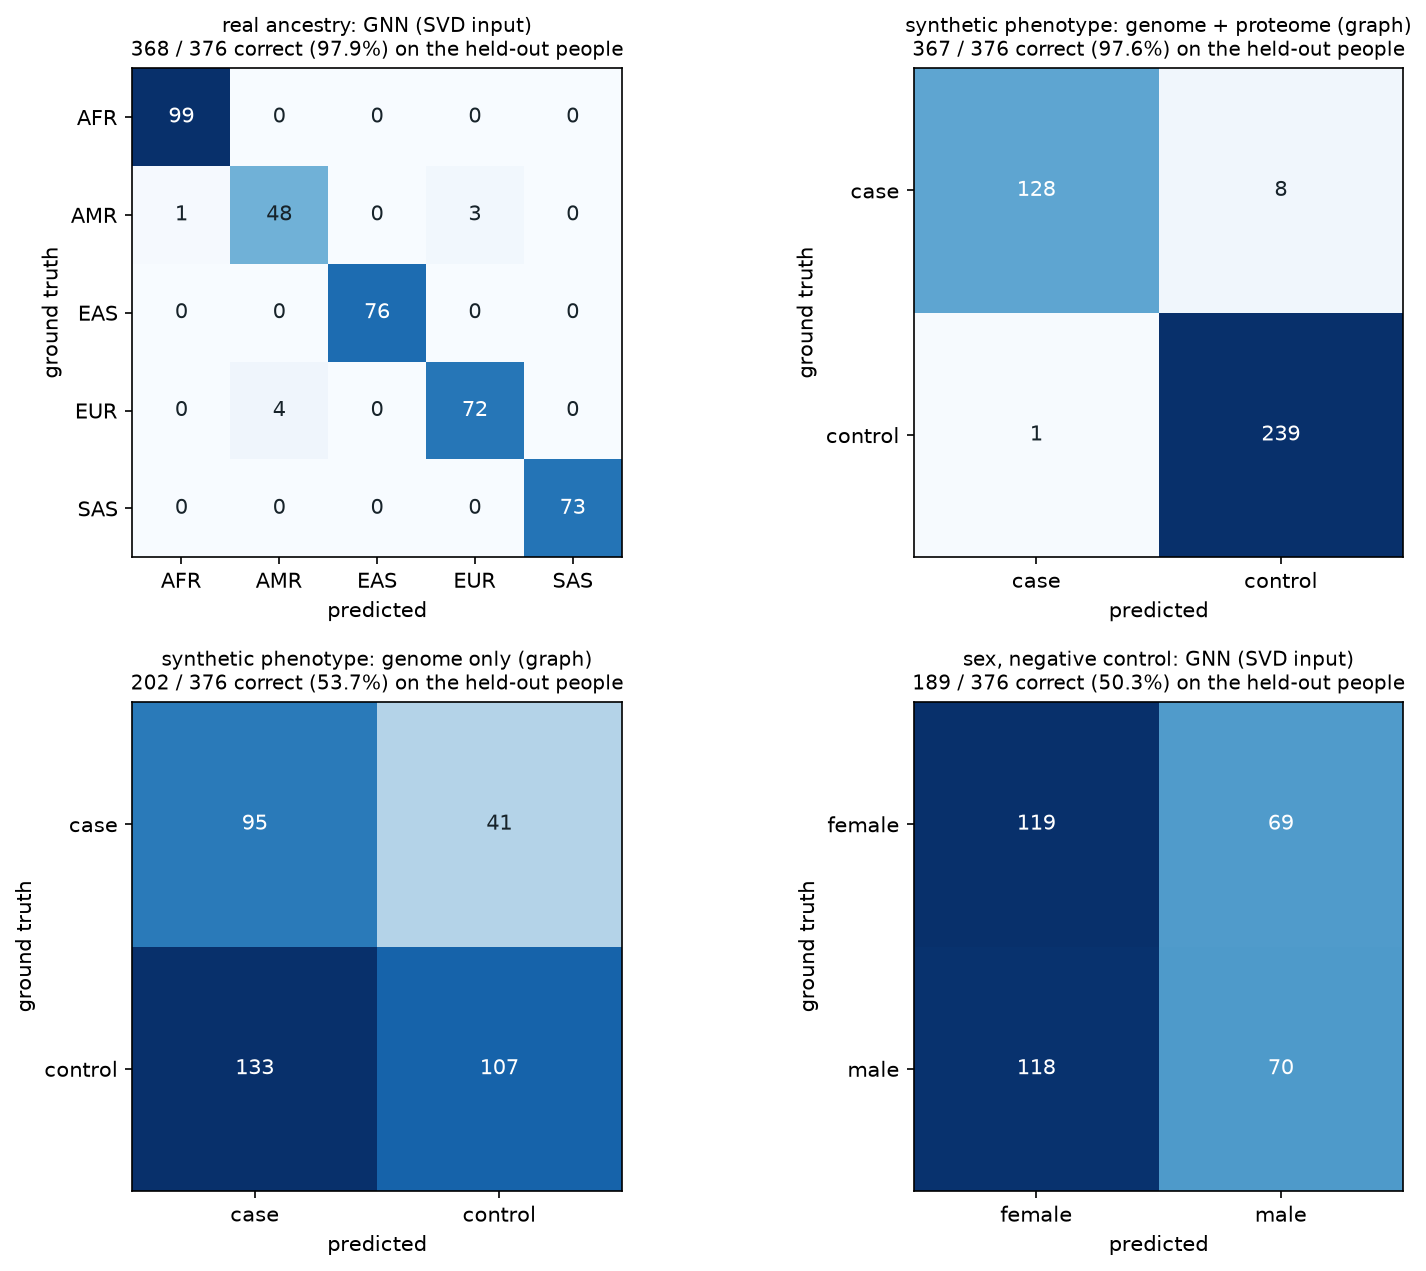
\includegraphics[width=0.95\linewidth]{confusion_matrices.png}
\caption{Ground truth versus prediction on the 376 held-out people: real ancestry (GNN, SVD input), the synthetic phenotype from genome plus proteome, from the genome alone, and sex, the negative control.}
\end{figure}

\begin{longtable}{p{0.329\linewidth}p{0.122\linewidth}p{0.122\linewidth}p{0.122\linewidth}p{0.122\linewidth}p{0.122\linewidth}}
\toprule
\textbf{Ancestry, true / predicted} & \textbf{AFR} & \textbf{AMR} & \textbf{EAS} & \textbf{EUR} & \textbf{SAS} \\
\midrule
\endhead
AFR (99) & 99 & 0 & 0 & 0 & 0 \\
AMR (52) & 1 & 48 & 0 & 3 & 0 \\
EAS (76) & 0 & 0 & 76 & 0 & 0 \\
EUR (76) & 0 & 4 & 0 & 72 & 0 \\
SAS (73) & 0 & 0 & 0 & 0 & 73 \\
\bottomrule
\end{longtable}

368 of 376 correct (balanced accuracy 0.974). The eight errors are all between AMR and EUR, which is what admixture predicts: the AMR panel populations carry European haplotypes.

\begin{longtable}{p{0.432\linewidth}p{0.122\linewidth}p{0.122\linewidth}p{0.263\linewidth}}
\toprule
\textbf{Synthetic phenotype, true / predicted} & \textbf{case} & \textbf{control} & \textbf{correct} \\
\midrule
\endhead
genome plus proteome (graph): case (136) & 128 & 8 & 367 / 376, AUC 0.992 \\
genome plus proteome (graph): control (240) & 1 & 239 &  \\
proteome only (MLP): case (136) & 129 & 7 & 364 / 376, AUC 0.962 \\
proteome only (MLP): control (240) & 5 & 235 &  \\
genome only (graph): case (136) & 95 & 41 & 202 / 376, AUC 0.601 \\
genome only (graph): control (240) & 133 & 107 &  \\
sex, negative control: female (188) & 119 & 69 & 189 / 376, chance \\
sex, negative control: male (188) & 118 & 70 &  \\
\bottomrule
\end{longtable}

The genome alone gets little more than half right because the planted genomic signal is 20 clusters through a noisy logistic link; the proteome carries most of the signal; the graph that joins the two makes the fewest errors, with a single false case. Sex on an autosome is a coin flip, as it must be.

\begin{longtable}{p{0.075\linewidth}p{0.470\linewidth}p{0.132\linewidth}p{0.263\linewidth}}
\toprule
\textbf{Rank} & \textbf{Cluster (saliency of the combined model)} & \textbf{Saliency} & \textbf{Planted causal cluster?} \\
\midrule
\endhead
1 & chr22\_46902935-46974137\_cluster186 & 0.110 & yes \\
2 & chr22\_44263132-44288496\_cluster19 & 0.080 & yes \\
3 & chr22\_25066667-25206817\_cluster346 & 0.077 & yes \\
4 & chr22\_46974137-47051453\_cluster43 & 0.055 & no \\
5 & chr22\_44166469-44185056\_cluster231 & 0.054 & yes \\
6 & chr22\_47257518-47285160\_cluster1 & 0.046 & no \\
7 & chr22\_40032702-40132216\_cluster25 & 0.046 & no \\
8 & chr22\_49408121-49430759\_cluster3 & 0.043 & no \\
9-20 & twelve further clusters & 0.042-0.036 & no \\
\bottomrule
\end{longtable}

Four of the top twenty (and the top three outright) are among the 20 planted causal clusters out of 6,551; by chance 0.06 would be. For the genome-to-protein direction the ridge finds 4 of the 20 cis proteins with test R-squared above 0.1 and none of the 440 others. The federated global model, scored on the same 376 people, reaches AUC 0.998 and balanced accuracy 0.963 against the central model's 0.992 and 0.969.

\subsection{Where the language model sits, and what it achieves}

The language model is not part of training and makes no prediction. It sits after the encoder, once per person, as the decoder: graphrag\_decoder.py walks the graph around one person and collects facts (their ancestry-informative clusters with blocks, genes and proteins; their most extreme protein levels and the block that encodes each; the GNN's prediction; the salient clusters they carry; their five nearest neighbours in the embedding), serialises them as JSON and asks the NIM model (nvidia/nemotron-3-super-120b-a12b) to write a structured report using only those facts and citing every id verbatim. The code then checks each cited id against the context. What this achieves is the last step the README's mission implies, turning numbers into an insight a research team can read: a summary, an ancestry assessment, a phenotype assessment, explicit genome-to-proteome links and caveats, each traceable to graph ids. For HG00103 (EUR, GBR, 994 clusters carried, predicted control) the model answered in 13 seconds from a 4,555-token context with a 1,020-token reply, cited 25 ids and invented none; its links named, for example, cluster chr22\_40032702-40132216\_cluster151 in the block encoding TNRC6B (protein Q9UPQ9) and cluster chr22\_26024448-26060666\_cluster35 in the block encoding MYO18B (Q8IUG5), and its caveats stated that the phenotype is synthetic and that ancestry is population structure, not a medical finding. Without an API key the same script prints the exact prompt (dry run), so the retrieval can be inspected offline.

\begin{longtable}{p{0.329\linewidth}p{0.611\linewidth}}
\toprule
\textbf{Retrieved fact for HG00103} & \textbf{Value} \\
\midrule
\endhead
GNN prediction & control (truth: control) \\
globally salient clusters carried & chr22\_46902935-46974137\_cluster186 (0.110), chr22\_46974137-47051453\_cluster43 (0.055), chr22\_40032702-40132216\_cluster25 (0.046) \\
most ancestry-informative clusters, with block genes and proteins & cluster151 of block 40032702-40132216 (TNRC6B, Q9UPQ9); cluster545 of 35738379-36060254 (RBFOX2, O43251); cluster35 of 26024448-26060666 (MYO18B, Q8IUG5) \\
most extreme protein levels (z) & H1-0 +2.75, RIMBP3 -2.65, INPP5J +2.53, CRYBA4 +2.52, YWHAH +2.37 \\
nearest people in the embedding & HG01767 (EUR), NA12842 (EUR), HG00351 (EUR), HG04002 (SAS), HG00336 (EUR) \\
\bottomrule
\end{longtable}

\begin{longtable}{p{0.207\linewidth}p{0.733\linewidth}}
\toprule
\textbf{Decoder field} & \textbf{Text returned (Nemotron 3 Super, 13.3 s, 25 ids cited, 0 unknown)} \\
\midrule
\endhead
summary & Individual HG00103 is of EUR ancestry (GBR population) and carries 994 haploblock clusters. The GNN phenotype prediction for this individual is 'control', which is a synthetic case/control label used for pipeline testing. Several ancestry-informative clusters are carried, showing high enrichment in various populations including EUR, EAS, and SAS. \\
ancestry\_assessment & The individual's ancestry is EUR (European) as per the 1000G panel data, with population label GBR. This reflects population structure, not a medical finding. \\
phenotype\_assessment & The GNN-predicted phenotype is 'control', which is a synthetic case/control label used to test the pipeline; it does not reflect a real medical condition. \\
genome\_proteome\_links & cluster151 $\rightarrow$ block 40032702-40132216 $\rightarrow$ TNRC6B $\rightarrow$ Q9UPQ9 (carried, enriched in EAS); cluster545 $\rightarrow$ RBFOX2 $\rightarrow$ O43251; cluster35 $\rightarrow$ MYO18B $\rightarrow$ Q8IUG5 (enriched in EUR) \\
caveats & ancestry is population structure, not a medical finding; the phenotype is synthetic; not all clusters have gene or protein annotations; the prediction comes from the embedding and may not match observed protein levels \\
\bottomrule
\end{longtable}

What the LLM adds is the sentence layer: a readable paragraph, the genome-to-protein chain spelled out per person, the right hedges attached automatically, graceful handling of missing information (for HG00096, who is not in the held-out split, it reported that no prediction exists instead of inventing one), and traceability, because every claim carries an id that the code verifies. It makes no prediction and adds no outside knowledge.

\subsection{Connecting the dots to the README on branch main}

The team README fixes a mission, three research questions, a chromosome-22 demo scope, five required datasets and a data-integration flowchart. Each maps to something concrete in genomics/:

\begin{longtable}{p{0.282\linewidth}p{0.423\linewidth}p{0.235\linewidth}}
\toprule
\textbf{README item} & \textbf{What it became} & \textbf{Evidence} \\
\midrule
\endhead
Mission: each institution keeps individual-level data locally, trains the same graph model, exchanges only model updates; a server aggregates and returns them & the person is its own node type, so a site holds only its people and their CARRIES and MEASURED edges while the cluster/block/gene/protein graph is public; NVFlare FedAvg with client.py sending a state dict only & outputs/federated/chr22/evaluation.json: AUC 0.998 vs central 0.992 \\
Opening line: a variant-based phenotype-propensity reference graph combined with patient-specific proteomics, what can we learn? & reference graph = the shared cluster/block/gene/protein layer; patient-specific = Individual nodes with CARRIES and MEASURED edges; learned: integration beats either modality alone, cis effects need sparse models, federation costs nothing when sites are alike & sections 9, 11, 13 \\
Background: one gene gives many protein products & 917 UniProt isoform rows collapsed to 460 proteins with an isoform count as a Protein feature; ENCODES keeps gene to protein explicit & haplokg\_proteins.load\_protein\_bed \\
RQ1: connect haploblock genomics to genes and proteomic data in a graph model & schema v2, five node types, seven edge types, one join key; the README flowchart maps one-to-one: Participant = Individual, Haploblock hash = Cluster, Haploblock = Block, Encoded protein = Gene ENCODES Protein, Measured abundance = MEASURED edge & section 6; Neo4j browser \\
RQ2: can a GNN combine genomic and proteomic information to identify disease-related phenotype clusters & yes, in both senses of cluster: groups of people (AUC 0.60 genome, 0.96 proteome, 0.99 both; embedding silhouette 0.70) and haploblock clusters tied to the phenotype (saliency top 3 all causal); the person-level graph, with every participant as a node, is what lets the GNN use both modalities & sections 8, 9; Part II ground truth tables \\
RQ3 (aspirational): train across institutions without transferring individual-level data & done in NVFlare simulation with three sites; real-machine POC is the next step & section 11 \\
Demo scope: chromosome 22 first & everything runs on chr22; nothing is chromosome-specific (CHROM=chr21 make run) & Makefile \\
Dataset 1: haploblock BED and per-individual haploblock hashes & boundaries and block\_stats from haploblocks.org; the hashes were already clustered upstream into the HaploGraph clusters we consume, so no hash was recomputed & fetch\_data.sh \\
Dataset 3: gene BED for chr22 & uniprot\_chr22.bed (team); Block OVERLAPS Gene by coordinate intersection, 1,063 edges, 29 genes outside every block & build\_kg\_v2.py \\
Dataset 4: gene-to-protein mapping & the same BED: UniProt accession per gene, isoforms collapsed; 460 ENCODES edges & build\_kg\_v2.py \\
Dataset 5: proteomic data for chr22 proteins & the team's 120-patient synthetic set validated the proteomics plumbing but cannot join the genome (its ids are not 1000G ids and its phenotype has no genomic cause); the joinable set on 2,503 real 1000G ids with ground truth replaces it for integration; real data (Wu 2013, UKB-PPP) is the planned next source & proteomics\_synth\_1000g.py \\
Data-integration flowchart & implemented as a PyTorch Geometric HeteroData object plus a Neo4j load, with two additions the README did not list: CO\_OCCURS between clusters and NEXT\_BLOCK between blocks & hetero\_v2.pt; neo4j\_load.py \\
\bottomrule
\end{longtable}

\section{Part III: The project}

\subsection{1. Problem statement and goal}

The team's README (branch main) states the mission: develop a proof-of-concept workflow that integrates a known genome graph with proteomics, with a federated approach where each participating institution retains its individual-level data locally and trains the same graph-based model, exchanging only model updates with a coordinating server. Three research questions make it concrete:

\begin{itemize}[leftmargin=1.4em]
  \item RQ1: How can haploblock-based genomic information be connected to genes and proteomic data in a graph-based data model?
  \item RQ2: Can a graph neural network combine genomic and proteomic information to identify disease-related phenotype clusters?
  \item RQ3 (aspirational): Can a graph neural network trained across multiple institutions predict clinical outcomes without transferring individual-level data?
\end{itemize}

Translated into engineering: build a typed graph in which a person links to the haplotype clusters they carry, clusters sit in blocks, blocks overlap genes, genes encode proteins, and the same person links to their measured protein levels (RQ1); train a GNN on it and show that genome plus proteome predicts a phenotype better than either alone while negative controls stay at chance (RQ2); split the people by site, share only the reference graph and the model weights, and show the federated model matches the central one (RQ3). The demo scope fixed by the team is chromosome 22.

What was already available: the mentor (Ben Busby) pointed the team to haploblocks.org, whose data server publishes a ready-made graph of haplotype clusters for the 1000 Genomes people, built for this hackathon at Rigshospitalet's MDxCORE unit. That is what "we don't have to build the genome graph" meant; everything downstream of it is ours.

\subsection{2. Data sources: what, where, why}

\begin{figure}[htbp]
\centering
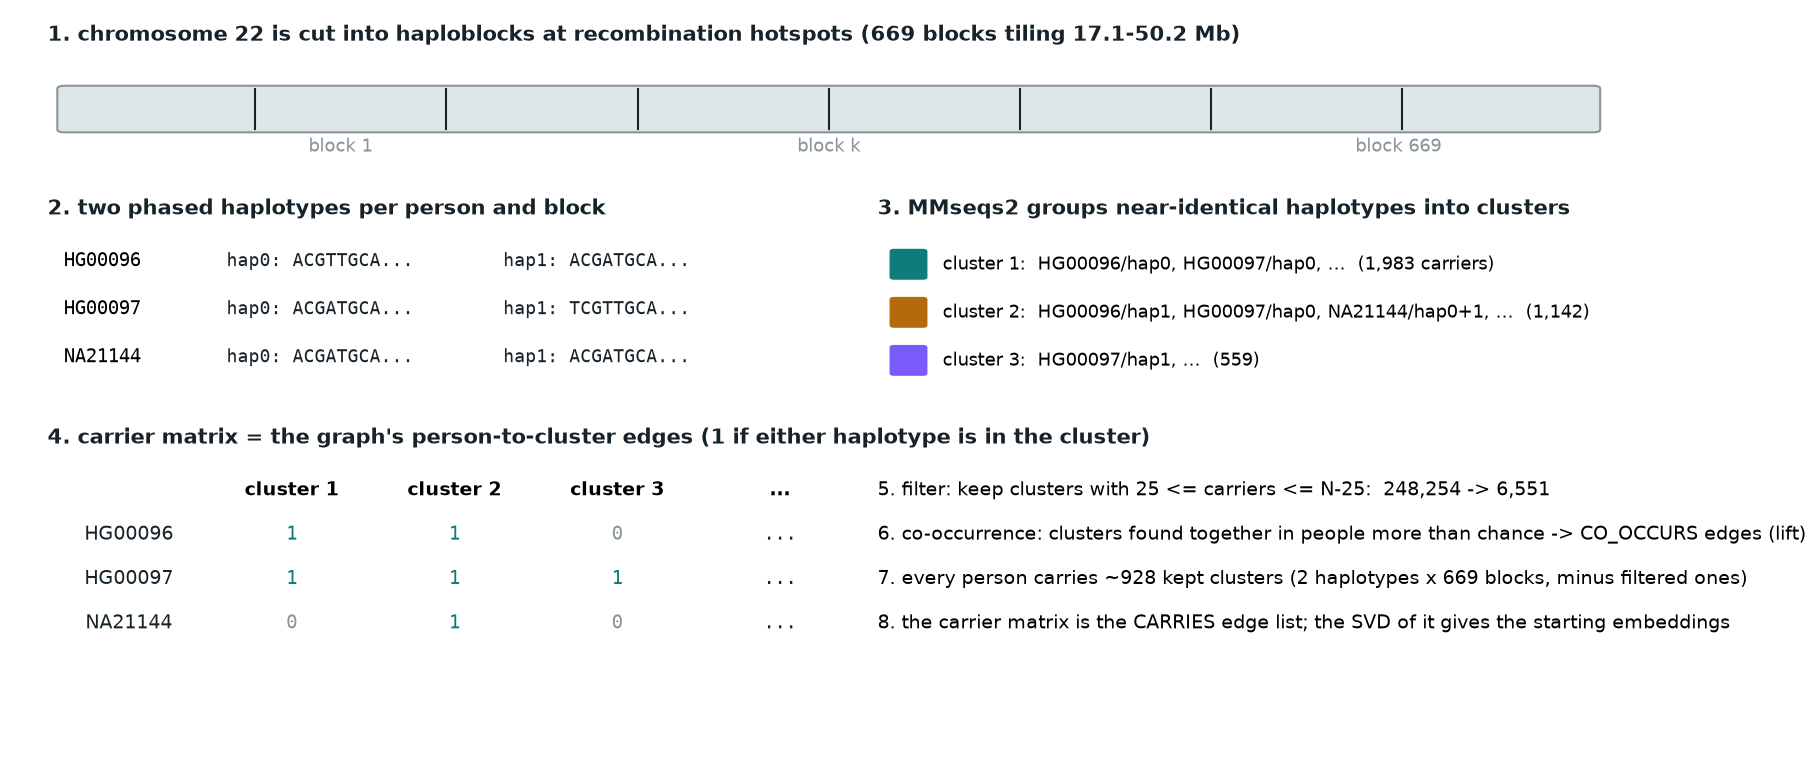
\includegraphics[width=0.95\linewidth]{genome_to_graph.png}
\caption{From genomes to a graph: blocks, phased haplotypes, MMseqs2 clusters, the carrier matrix and the filters that produce the 6,551 kept clusters.}
\end{figure}

\begin{longtable}{p{0.188\linewidth}p{0.207\linewidth}p{0.282\linewidth}p{0.263\linewidth}}
\toprule
\textbf{Data} & \textbf{Where it comes from} & \textbf{What it contains} & \textbf{Why we use it} \\
\midrule
\endhead
HaploGraph nodes (nodes.csv.gz) & data.haploblocks.org/haplograph/1000G/chr22 & 248,254 haplotype clusters x 2,548 people; 1 if the person carries the cluster & The genome graph's node features; becomes our person-to-cluster edges \\
HaploGraph edges (edges\_lift\_above\_threshold.csv.gz) & same server & 187,030 cluster pairs that co-occur in people more than chance (lift $\geq$ 5), with weight and lift & Co-occurrence structure; the raw edges.csv is dominated by one near-universal haplotype and is not used \\
Block statistics (block\_stats.tsv, boundaries) & same server & 669 blocks on chr22: coordinates, length, number of clusters, entropy, dominance, singletons & Block nodes and their features \\
Phenotypes (phenotypes\_real.csv) & 1000G panel via IGSR, republished with the graph & ancestry, population, sex for 2,503 of the 2,548 people & The only real labels that exist; ancestry and population are targets, sex is the negative control \\
Protein coordinates (uniprot\_chr22.bed) & UCSC UniProt track, prepared by Friederike & 917 protein isoform rows $\rightarrow$ 460 proteins, 458 genes, with genomic spans & Block-to-gene overlaps and gene-to-protein mapping in one file \\
Synthetic proteomics, team version & proteomics/generate\_synthetic\_proteomics.py (Nolan; regenerated on main with 4,000 samples) & 3 sites, first 40 then 1,333-1,334 patients each (ids SITE1\_PT0001...), age, sex, case/control, log2 intensities for 460 proteins & The team's proteomics analyses on main run on it; for the genome join a version keyed to 1000G ids was needed (next row) \\
Synthetic proteomics, joinable version & genomics/proteomics\_synth\_1000g.py (this work) & 2,503 real 1000G ids, 3 mixed-ancestry sites, phenotype driven by 20 causal clusters, cis effects, batch shift, missingness; ground truth saved & Lets the integration be scored against a known answer \\
Planned real proteomics & Wu et al. 2013 (Nature): 95 HapMap LCLs with 1000G ids; UKB-PPP pQTL summary statistics on AWS Open Data & per-person protein levels; variant-to-protein effect sizes & Real join on the same ids; real cluster-to-protein propensity edges \\
\bottomrule
\end{longtable}

How the genome graph was made upstream (haploblocks.org pipeline, Kubica et al. 2025): (1) recombination-rate peaks define haploblocks; (2) each person's two phased haplotype sequences are cut out per block from the 1000G VCF; (3) all haplotypes of a block are merged into one FASTA; (4) MMseqs2 clusters near-identical haplotypes, giving each haplotype a cluster id; (5) a compact hash encodes strand, chromosome, block, cluster and variants. A sixth step (haploblock-graph-builder) produced the HaploGraph: nodes are clusters, the node feature is the 0/1 vector over people, edges join clusters that co-occur in the same people. We did not rerun these steps; we verified their outputs agree (669 blocks in every file, identical per-block cluster counts in all 669, 248,254 clusters both ways) and consumed them.

\subsection{3. The data pipeline}

\begin{figure}[htbp]
\centering
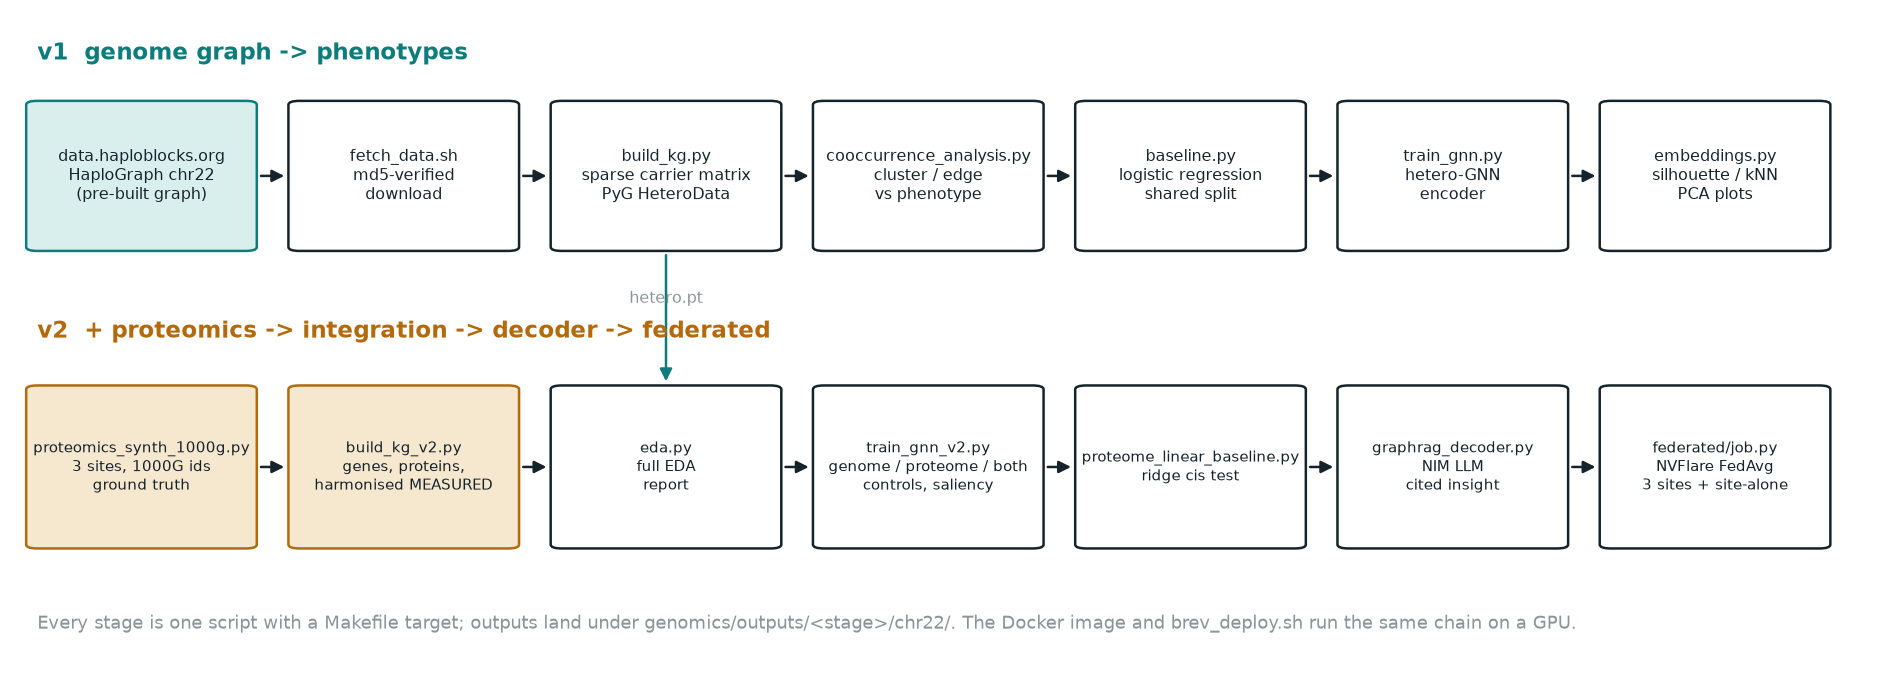
\includegraphics[width=0.95\linewidth]{workflow_pipeline.png}
\caption{The two pipeline chains (v1 genome graph, v2 proteomics integration), one script per stage.}
\end{figure}

Everything is a numbered script under genomics/, driven by a Makefile so a fresh clone runs with two commands. Downloaded inputs and generated outputs are git-ignored and regenerated; secrets are read from environment variables and never stored in the repository.

\begin{longtable}{p{0.066\linewidth}p{0.235\linewidth}p{0.423\linewidth}p{0.216\linewidth}}
\toprule
\textbf{Step} & \textbf{Script} & \textbf{What it does} & \textbf{Output} \\
\midrule
\endhead
1 & fetch\_data.sh & downloads the chr22 HaploGraph files, phenotypes, block statistics; verifies md5 checksums & data/ \\
2 & build\_kg.py (haplokg.py) & streams nodes.csv.gz as int8 in 8,192-row chunks into a sparse matrix; filters clusters; joins phenotypes; maps edges; writes tables and the PyG graph & outputs/kg/chr22/ (carries.npz, hetero.pt) \\
3 & cooccurrence\_analysis.py & cluster x phenotype tests, edge x phenotype similarity, per-block informativeness, plots & outputs/cooccurrence/chr22/ \\
4 & baseline.py & logistic regression on the carrier matrix; writes the shared train/val/test split & outputs/baseline/, outputs/splits/ \\
5 & graph\_explore.py & NetworkX statistics, GraphML export, region and chromosome-wide plots & outputs/graph/chr22/ \\
6 & train\_gnn.py & the genome-only GNN with SVD / Node2Vec / learned / raw inputs & outputs/gnn/chr22/ \\
7 & embeddings.py & quality of SVD and GNN embeddings: silhouette, nearest-neighbour accuracy, PCA plots & outputs/embeddings/chr22/ \\
v2.1 & proteomics\_synth\_1000g.py & synthetic proteomics on the real 1000G ids with saved ground truth & outputs/proteomics\_synth/chr22/ \\
v2.2 & build\_kg\_v2.py (haplokg\_proteins.py) & adds genes, proteins, block-gene overlaps, harmonised measurements & outputs/kg/chr22/hetero\_v2.pt \\
v2.3 & eda.py & the full exploratory report with tables and plots & outputs/eda/chr22/EDA.md \\
v2.4 & train\_gnn\_v2.py & genome / proteome / both ablations, controls, saliency, proteome regression & outputs/gnn\_v2/chr22/ \\
v2.5 & proteome\_linear\_baseline.py & per-protein ridge: can the genome predict each protein? & outputs/gnn\_v2/chr22/proteome\_ridge\_baseline/ \\
v2.6 & graphrag\_decoder.py & graph retrieval + NVIDIA NIM LLM $\rightarrow$ cited insight per person & outputs/graphrag/chr22/ \\
v2.7 & federated/job.py, client.py, model.py, evaluate\_global.py & NVFlare FedAvg over 3 sites and central scoring of the global model & outputs/federated/chr22/ \\
- & infer.py & inference benchmark: eager vs torch.compile vs TensorRT & outputs/gnn/.../inference/ \\
- & neo4j\_load.py, docker-compose.yml & loads the graph into Neo4j for browsing & localhost:7474 \\
\bottomrule
\end{longtable}

Memory arithmetic that shaped step 2: the node file is 1.3 GB as text; as a dense 64-bit matrix it would be 5 GB, as dense int8 632 MB, as a sparse matrix with 2.8 million non-zeros about 30 MB. Streaming chunks into sparse form keeps the whole build under 1 GB and 26 seconds on a laptop.

The cluster filter: a cluster is kept if between 25 and N-25 people carry it (N = 2,548). A cluster carried by 2,540 people is as uninformative as one carried by 8; both have only 8 people on the informative side. This mirrors the HaploGraph's own symmetric edge filter and reproduces its node set exactly: 248,254 clusters become 6,551 and not one of the 187,030 edges loses an endpoint. 176,903 of the dropped clusters are singletons (one haplotype).

\subsection{4. Exploratory data analysis}

The EDA report (outputs/eda/chr22/EDA.md, generated by eda.py) has eight sections: provenance, individuals, haploblocks, clusters, co-occurrence, genes and proteins, proteomics, genome-proteome. The key measurements:

\begin{longtable}{p{0.188\linewidth}p{0.752\linewidth}}
\toprule
\textbf{Aspect} & \textbf{Measurement} \\
\midrule
\endhead
Individuals & 2,548 people; 2,503 labelled (AFR 660, EAS 504, EUR 503, SAS 489, AMR 347), 45 unlabelled kept as nodes; 26 populations of 61-113 people; sex balanced within each ancestry; split train 1,752 / val 375 / test 376 \\
Blocks & 669 tiling 17.1-50.2 Mb with no gaps; length median 29.7 kb (5-95\%: 8.9-151 kb, longest 775 kb); clusters per block median 214, max 2,806; singleton rate median 0.62; entropy median 3.15; longer blocks hold more clusters (Spearman 0.37) \\
Clusters & 6,551 kept of 248,254; each person carries \textasciitilde{}928 (two haplotypes x 669 blocks minus filtered); the person x cluster matrix is 14\% dense \\
Co-occurrence edges & 187,030 with lift $\geq$ 5 (median 5.5, max 76); only 121 join clusters of the same block; median distance between endpoints tens of Mb; 4,344 clusters have at least one edge; degree up to 358; the top hubs are all AFR-enriched rare clusters (the mega-hub artefact) \\
Genes / proteins & 458 genes, 460 proteins, 1,063 block-gene overlaps; 29 genes outside every block (chromosome ends and gaps); 117 genes span two blocks; up to 14 genes in one block \\
Proteomics (synthetic) & 2,503 people x 460 proteins, 3 sites of \textasciitilde{}835; log2 range 4.9-17.0; 7.4\% missing overall, up to 16\% for the least abundant proteins (missing-not-at-random at the detection limit); between-site shift 0.48 log2 before harmonisation, 0.00 after; 227 proteins keep a phenotype association at FDR 5\% \\
Genome-proteome & for the 20 ground-truth causal clusters, the correlation between carrying the cluster and its cis protein gives r-squared up to 0.54, mean 0.17, 10 of 20 above 0.1 - the ceiling any genome-to-proteome model can reach on this data \\
\bottomrule
\end{longtable}

\begin{figure}[htbp]
\centering
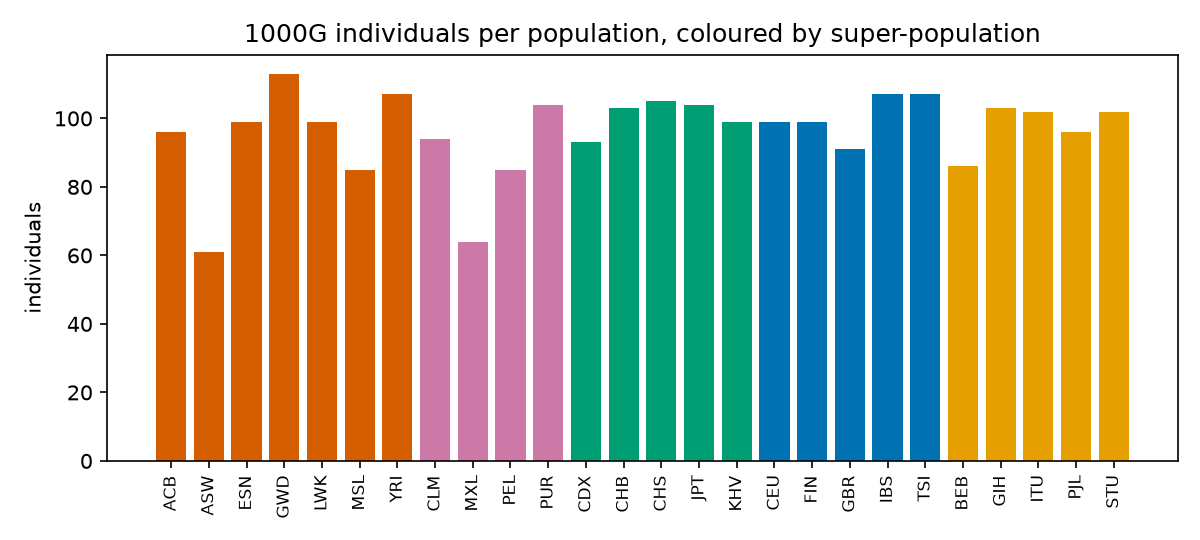
\includegraphics[width=0.90\linewidth]{eda_populations.png}
\caption{1000G individuals per population, coloured by continental ancestry.}
\end{figure}

\begin{figure}[htbp]
\centering
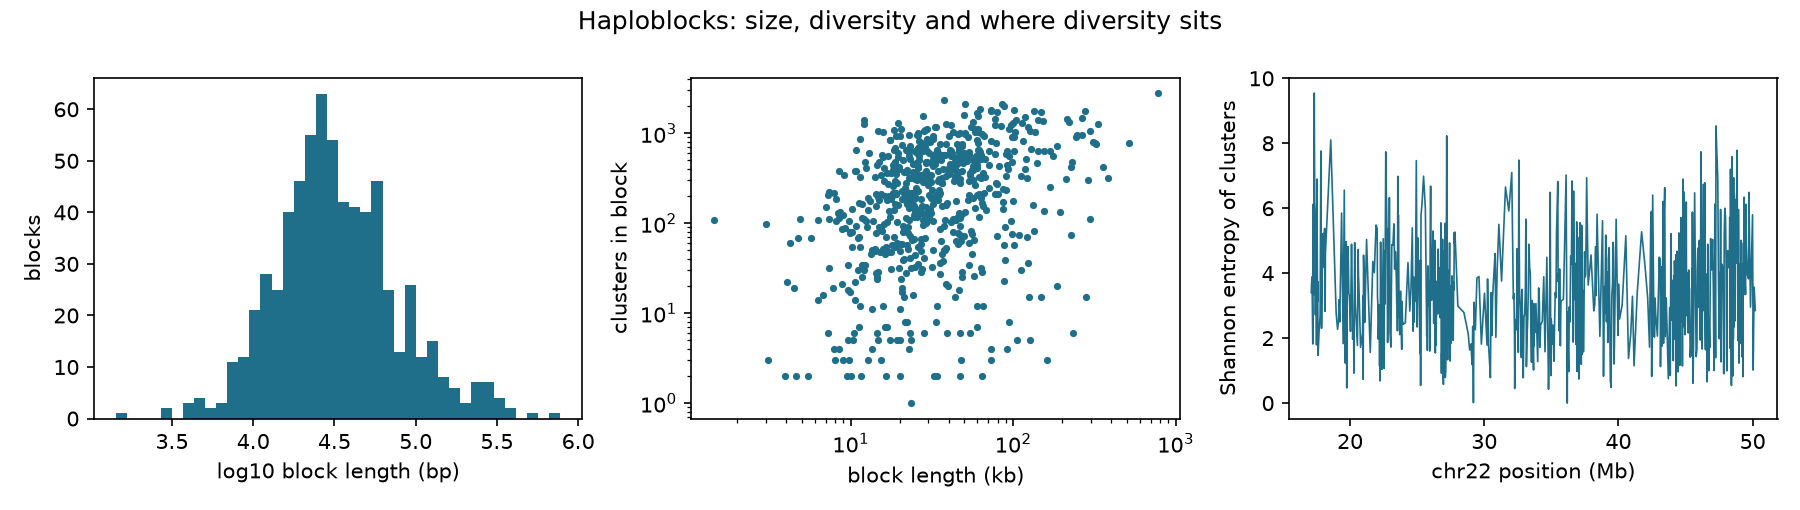
\includegraphics[width=0.95\linewidth]{eda_blocks.png}
\caption{Haploblocks on chr22: length distribution, clusters per block versus length, Shannon entropy of clusters along the chromosome.}
\end{figure}

\begin{figure}[htbp]
\centering
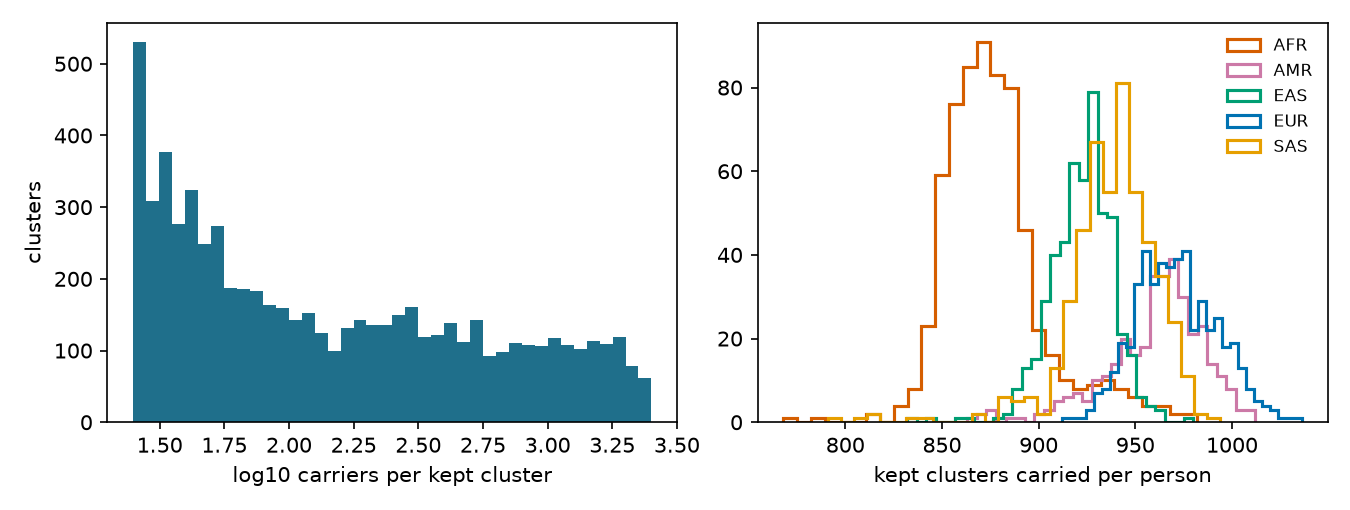
\includegraphics[width=0.90\linewidth]{eda_clusters.png}
\caption{Kept clusters: carriers per cluster (log scale) and clusters carried per person by ancestry.}
\end{figure}

\begin{figure}[htbp]
\centering
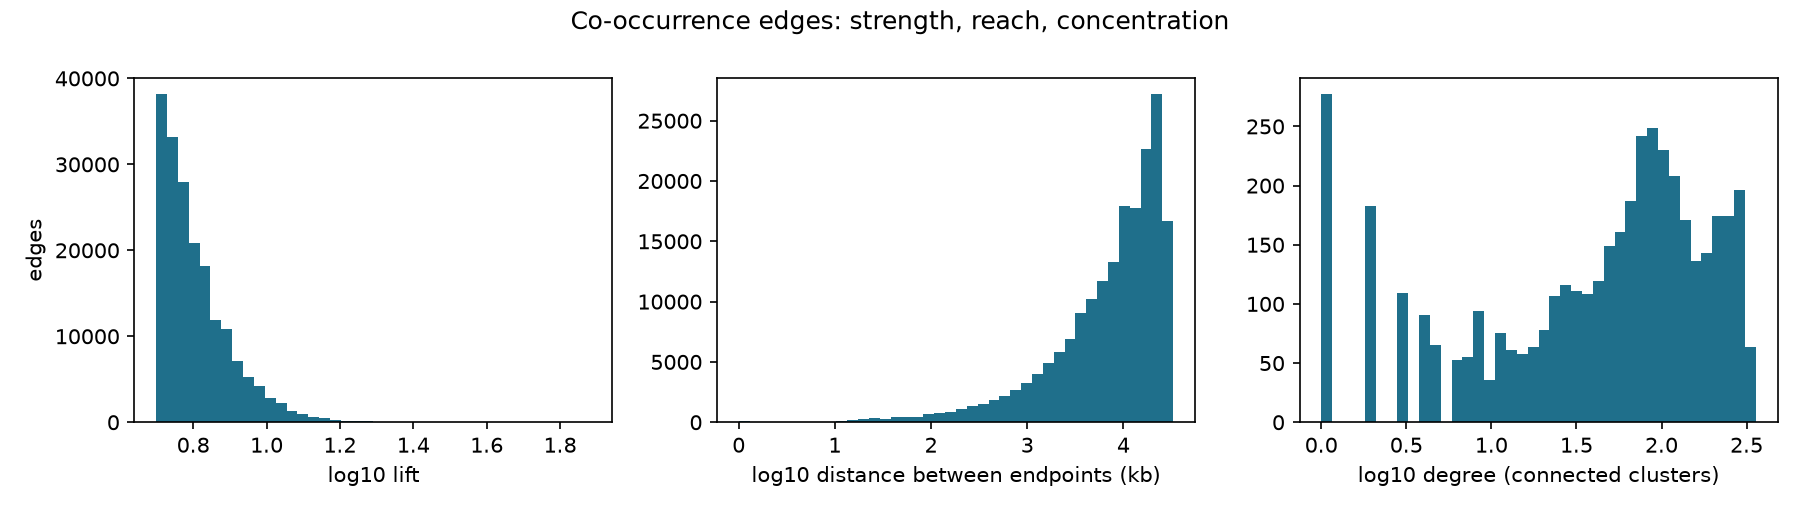
\includegraphics[width=0.95\linewidth]{eda_cooccurrence.png}
\caption{Co-occurrence edges: lift, distance between endpoints, degree.}
\end{figure}

\begin{figure}[htbp]
\centering
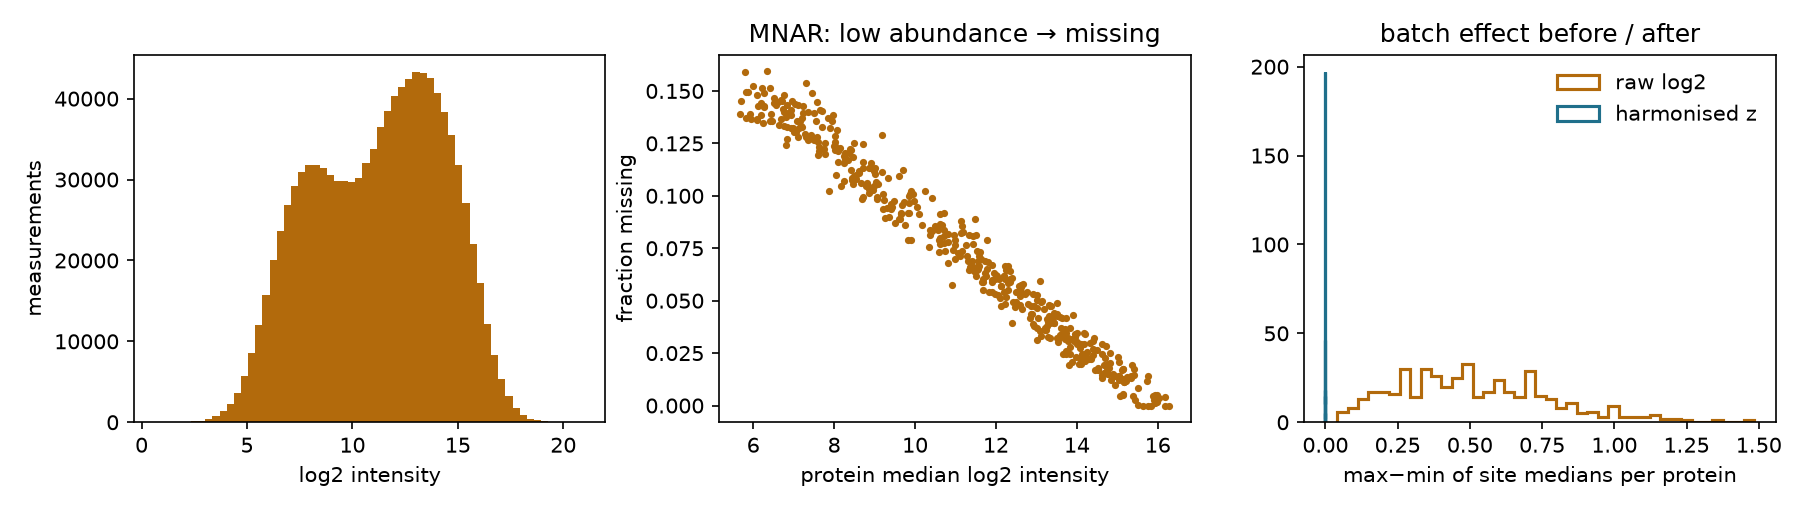
\includegraphics[width=0.95\linewidth]{eda_proteomics.png}
\caption{Synthetic proteomics: intensity distribution, missingness rising for low-abundance proteins, batch effect between sites before and after the harmoniser.}
\end{figure}

\begin{figure}[htbp]
\centering
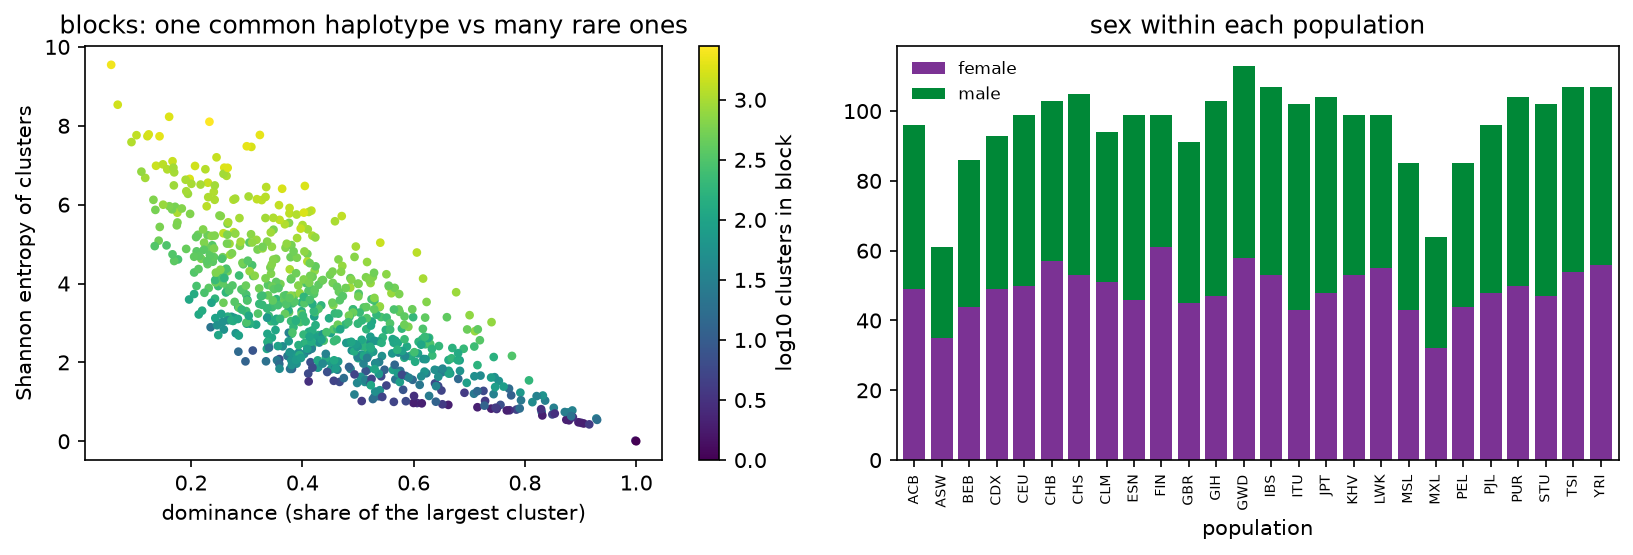
\includegraphics[width=0.95\linewidth]{eda_blocks_populations.png}
\caption{Blocks with one dominant haplotype versus many rare ones (left); sex within each of the 26 populations (right).}
\end{figure}

\begin{figure}[htbp]
\centering
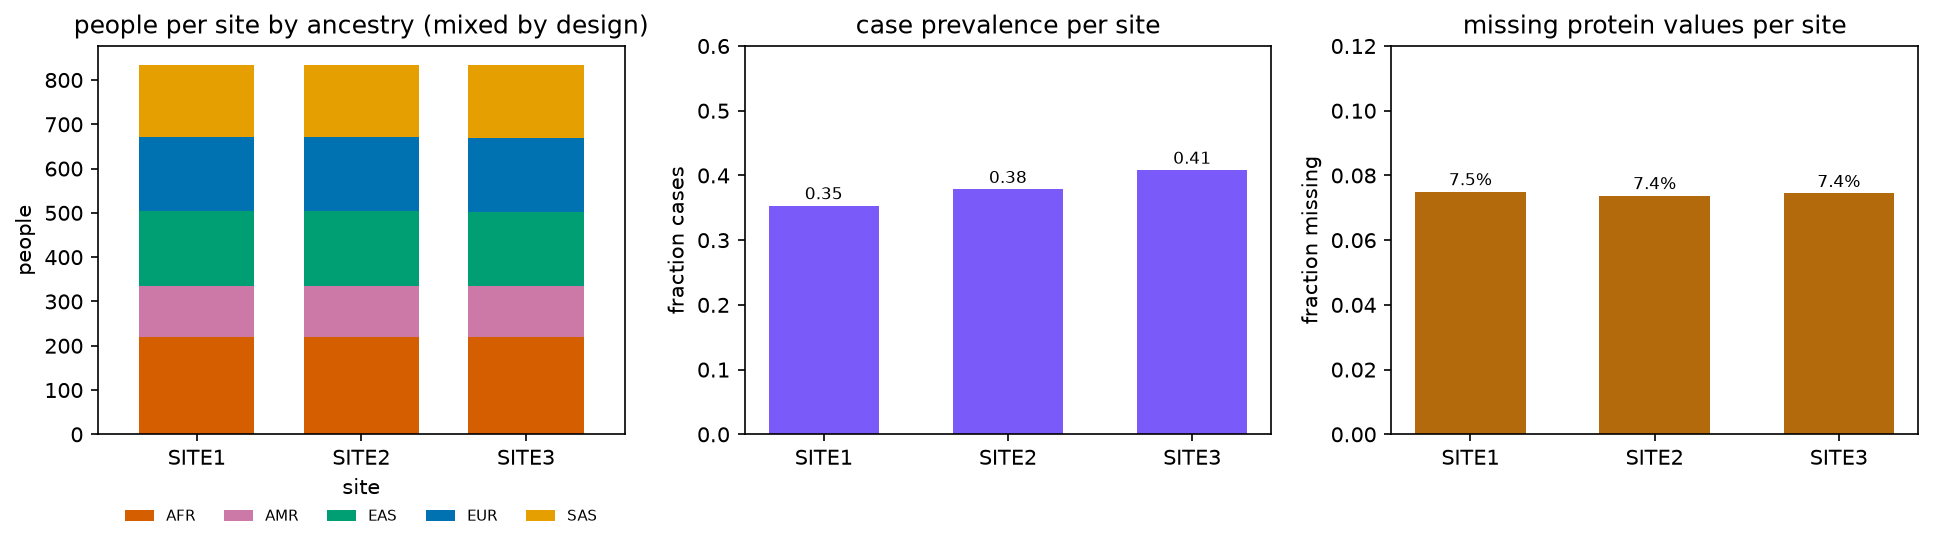
\includegraphics[width=0.95\linewidth]{sites_composition.png}
\caption{The three federated sites: people per site by ancestry (mixed by design), case prevalence per site, missing protein values per site.}
\end{figure}

\begin{figure}[htbp]
\centering
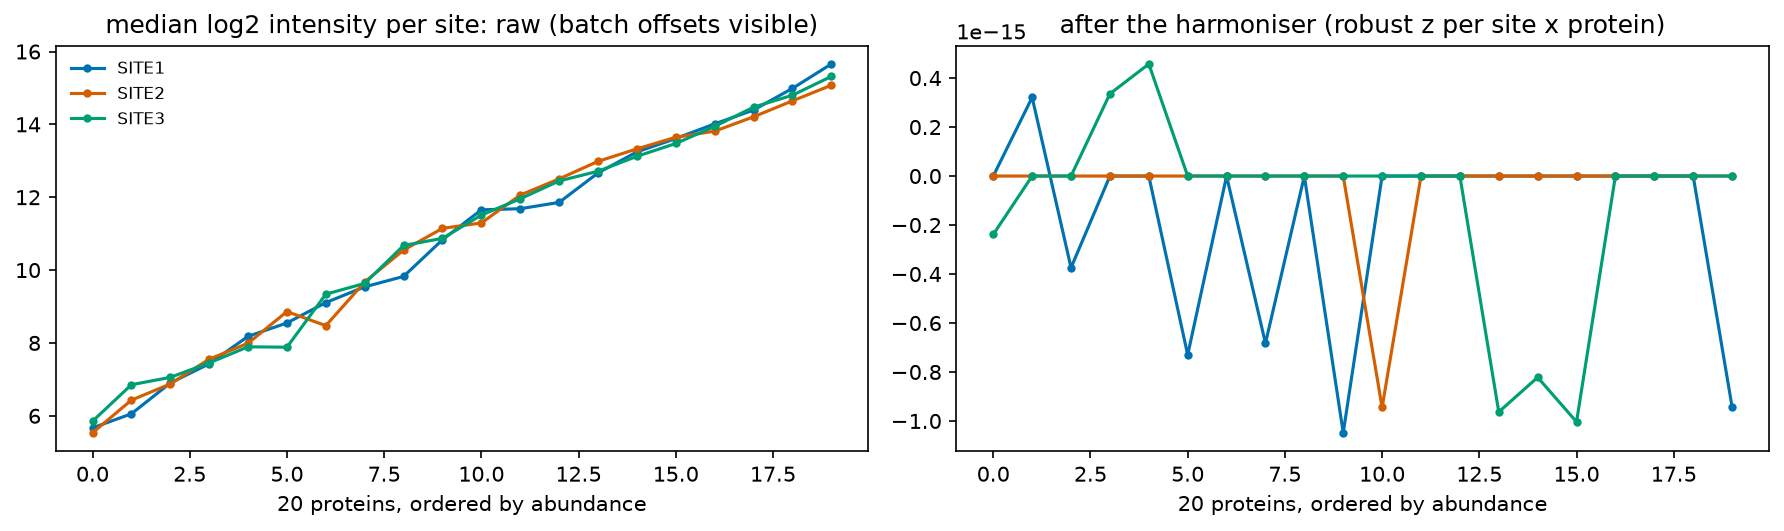
\includegraphics[width=0.95\linewidth]{sites_batch_effect.png}
\caption{Per-site protein medians before and after the harmoniser: the batch offsets vanish.}
\end{figure}

\begin{figure}[htbp]
\centering
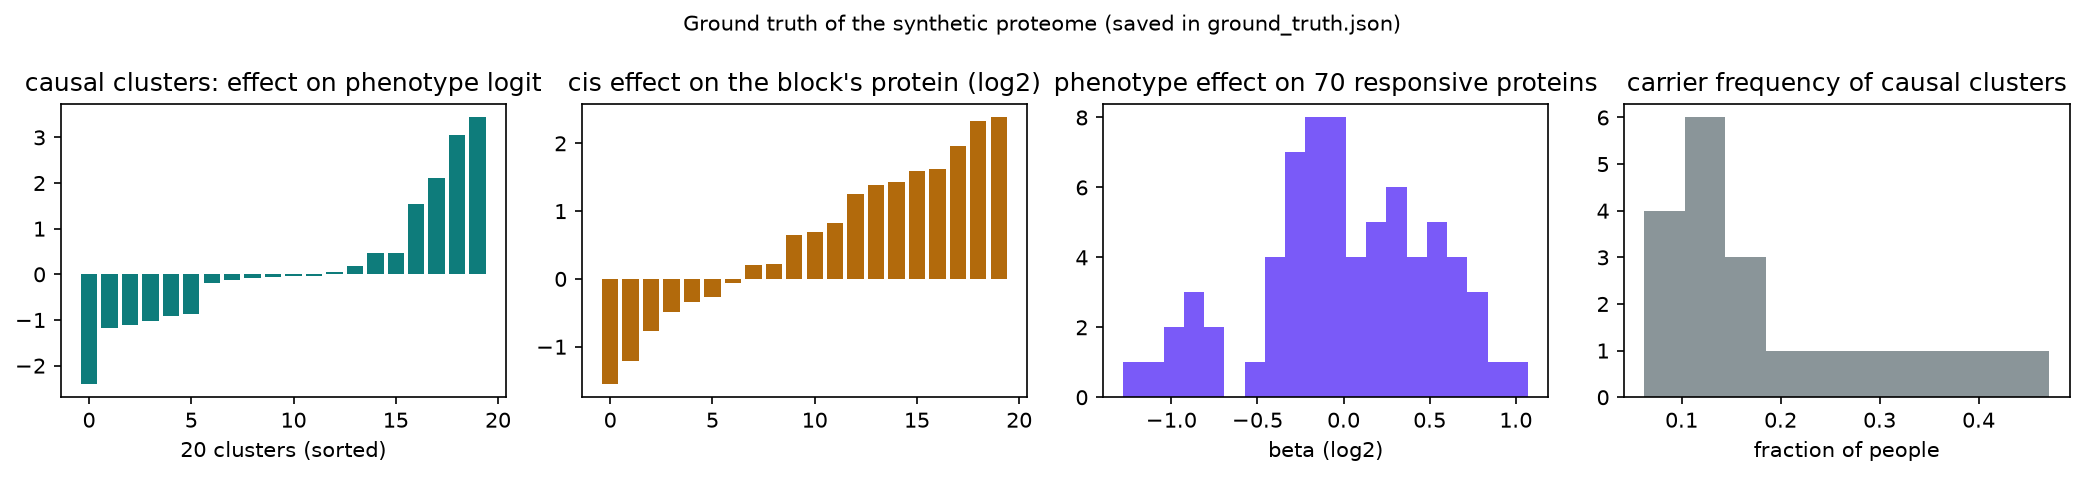
\includegraphics[width=0.95\linewidth]{ground_truth_effects.png}
\caption{Ground truth of the synthetic proteome: causal-cluster effects on the phenotype, cis effects on proteins, phenotype effects on the 70 responsive proteins, carrier frequencies of the causal clusters.}
\end{figure}

\subsection{5. Statistics: does the graph co-occur with phenotypes?}

Before any model we asked whether the graph carries phenotype information at all. For every cluster and each label we built the 2 x k table of carrier status versus class and computed a chi-square test with Cramer's V (a 0-1 effect size; for a 2 x k table V = sqrt(chi-square / N)), then Benjamini-Hochberg false-discovery-rate correction. All 6,551 tests run in one sparse matrix product.

\begin{itemize}[leftmargin=1.4em]
  \item Ancestry: 6,470 of 6,551 clusters (98.8\%) are associated at FDR 5\%; median V 0.20, maximum 0.81.
  \item Population: 6,378 clusters (97.4\%).
  \item Sex: 0 clusters; median V 0.013, maximum 0.03. This is the negative control: chr22 is autosomal, so a method that found sex signal would be fitting noise.
\end{itemize}

For the edges we compared the two endpoint clusters' ancestry-enrichment profiles: cosine similarity 0.86 for real edges versus 0.22 for degree-preserving shuffled pairs; 86\% of edges join clusters enriched in the same ancestry (42\% expected), and the similarity rises with lift (0.84 in the lowest lift quartile to 0.90 in the highest). Interpretation: the co-occurrence graph is largely population structure, long-range co-inheritance within ancestries rather than physical linkage.

\begin{figure}[htbp]
\centering
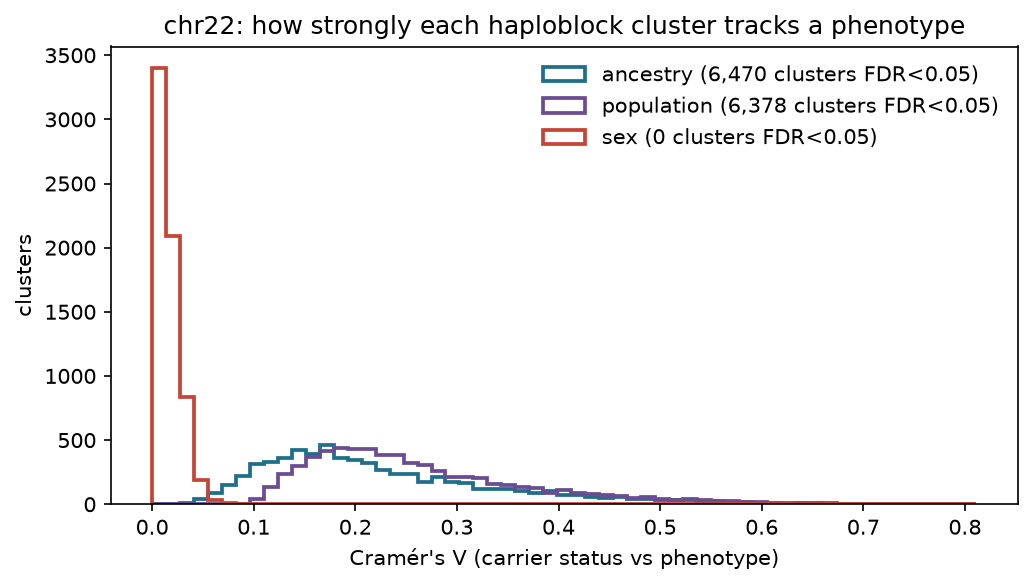
\includegraphics[width=0.85\linewidth]{cramers_v.png}
\caption{How strongly each cluster tracks a phenotype: ancestry and population carry signal, sex (the control) does not.}
\end{figure}

\begin{figure}[htbp]
\centering
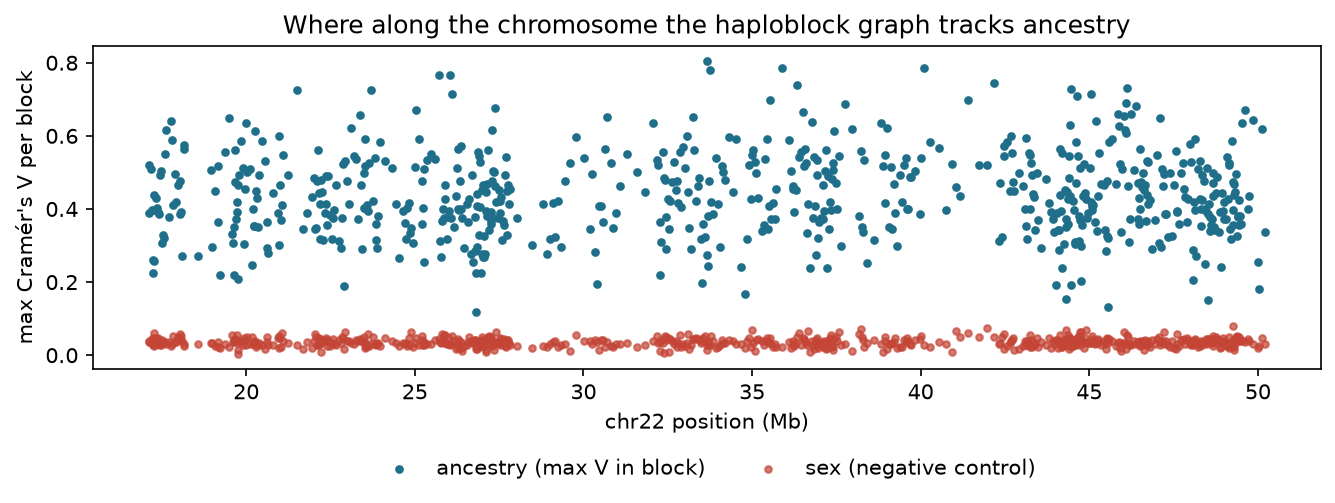
\includegraphics[width=0.95\linewidth]{informativeness.png}
\caption{Maximum Cramer's V per block along chr22 for ancestry versus sex.}
\end{figure}

\begin{figure}[htbp]
\centering
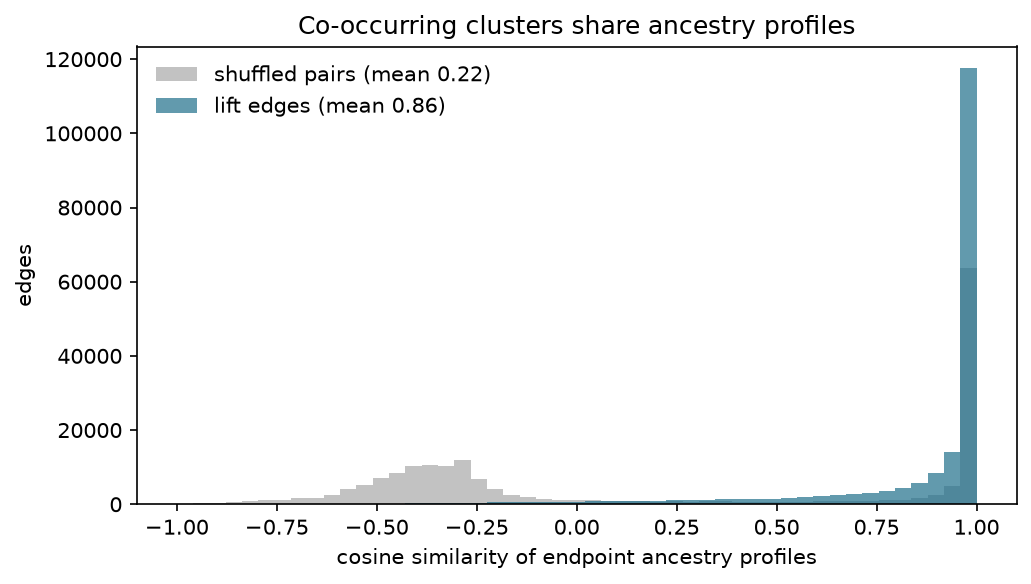
\includegraphics[width=0.85\linewidth]{edge_similarity.png}
\caption{Co-occurring clusters share ancestry profiles: real lift edges versus shuffled pairs.}
\end{figure}

\begin{figure}[htbp]
\centering
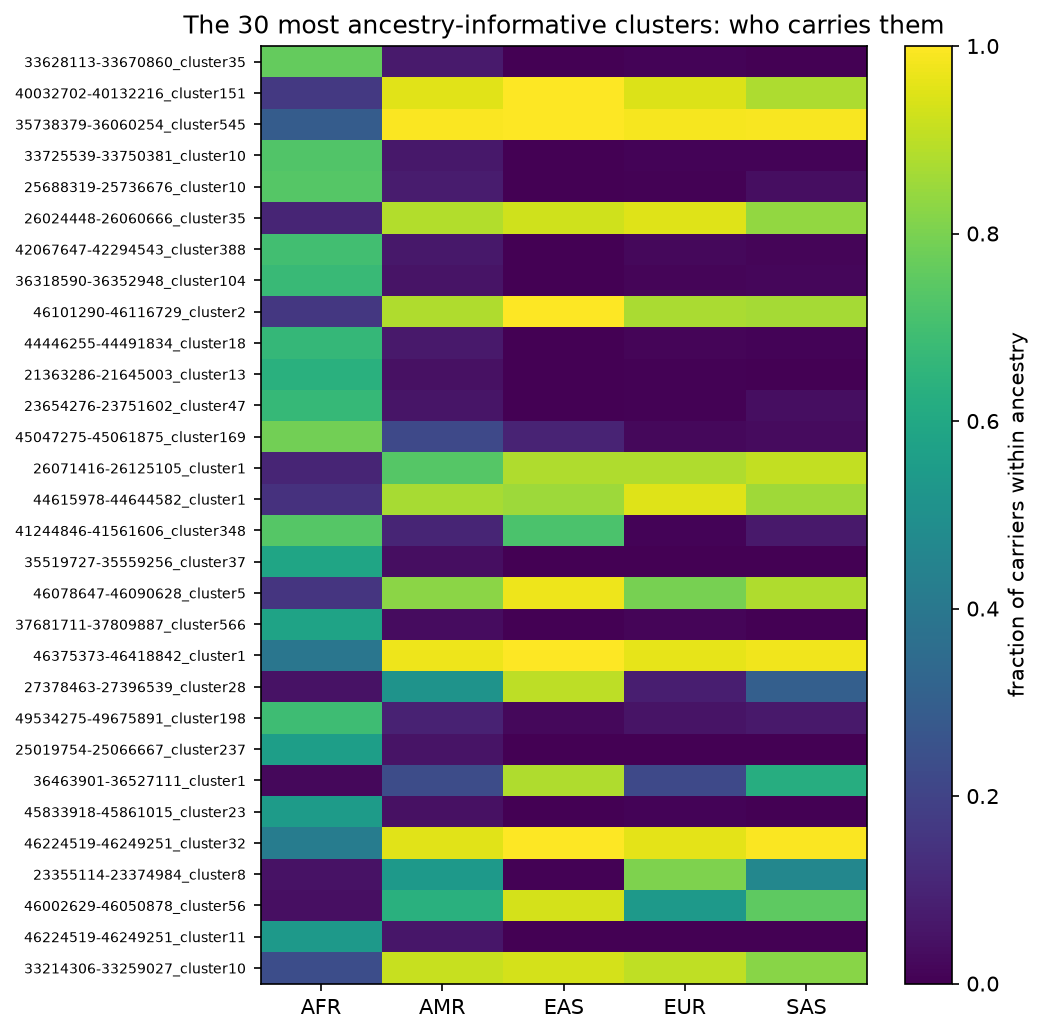
\includegraphics[width=0.60\linewidth]{informative_clusters_heatmap.png}
\caption{The 30 most ancestry-informative clusters and the fraction of each ancestry that carries them.}
\end{figure}

\subsection{6. The knowledge graph}

\begin{figure}[htbp]
\centering
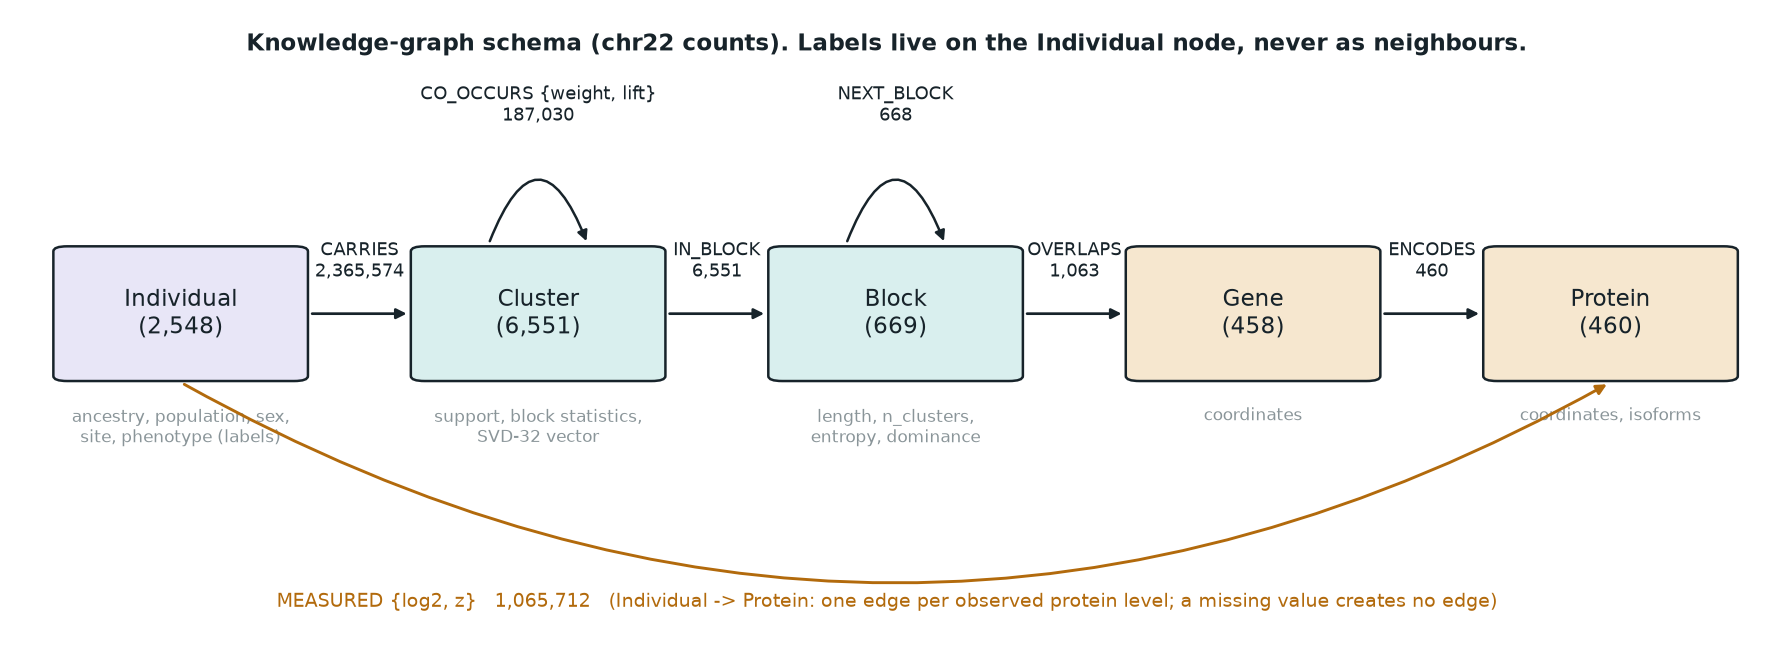
\includegraphics[width=0.95\linewidth]{schema_diagram.png}
\caption{Node and edge types of the knowledge graph with chr22 counts.}
\end{figure}

The HaploGraph has a single node type (cluster) and carries people only as a feature vector. We turned that vector into a second node type, the person, because a person is what phenotypes and protein measurements belong to, and what a hospital owns. The join is the 1000G sample id: the same string (for example HG00096) is a column header in nodes.csv.gz, a row key in phenotypes\_real.csv and a column in the proteomics matrices.

\begin{longtable}{p{0.141\linewidth}p{0.376\linewidth}p{0.113\linewidth}p{0.310\linewidth}}
\toprule
\textbf{Node type} & \textbf{Properties} & \textbf{Count} & \textbf{Source} \\
\midrule
\endhead
Individual & ancestry, population, sex, site, phenotype, age & 2,548 & nodes.csv.gz columns + phenotypes + proteomics metadata \\
Cluster & support, block statistics, SVD vector & 6,551 & nodes.csv.gz rows after the filter \\
Block & length, n\_clusters, entropy, dominance, singleton rate & 669 & block\_stats.tsv \\
Gene & coordinates, number of proteins & 458 & uniprot\_chr22.bed \\
Protein & coordinates, number of isoforms & 460 & uniprot\_chr22.bed \\
\bottomrule
\end{longtable}

\begin{longtable}{p{0.329\linewidth}p{0.470\linewidth}p{0.141\linewidth}}
\toprule
\textbf{Edge type} & \textbf{Meaning} & \textbf{Count} \\
\midrule
\endhead
Individual -CARRIES$\rightarrow$ Cluster & the person carries this haplotype cluster (the 1s of the matrix) & 2,365,574 \\
Cluster -CO\_OCCURS\{weight, lift\}$\rightarrow$ Cluster & the two clusters co-occur in people more than chance & 187,030 \\
Cluster -IN\_BLOCK$\rightarrow$ Block; Block -NEXT\_BLOCK$\rightarrow$ Block & position on the chromosome & 6,551; 668 \\
Block -OVERLAPS$\rightarrow$ Gene; Gene -ENCODES$\rightarrow$ Protein & coordinate intersection; protein product & 1,063; 460 \\
Individual -MEASURED\{log2, z\}$\rightarrow$ Protein & one edge per observed protein level; missing values create no edge & 1,065,712 \\
\bottomrule
\end{longtable}

Two design rules matter. First, phenotypes are properties of the person node, never nodes or edges: if a Phenotype node were connected to the person, a two-layer GNN would read the label from its neighbour and report a meaningless 100\%. Second, because people are their own node type, the site boundary is a clean cut: the cluster, block, gene and protein graph is public and identical at every site, while a site holds only its people and their CARRIES and MEASURED edges.

The graph is stored as a PyTorch Geometric HeteroData object (hetero.pt, hetero\_v2.pt) for modelling and loaded into Neo4j community edition (docker compose up neo4j; neo4j\_load.py) for browsing at localhost:7474, where a query such as MATCH (i:Individual \{id:'HG00096'\})-[:CARRIES]$\rightarrow$(c:Cluster)-[:IN\_BLOCK]$\rightarrow$(b:Block) RETURN i,c,b shows a person's haplotypes with their blocks. NetworkX (with the nx-cugraph GPU backend in the image) produces statistics and GraphML for Gephi.

\begin{figure}[htbp]
\centering
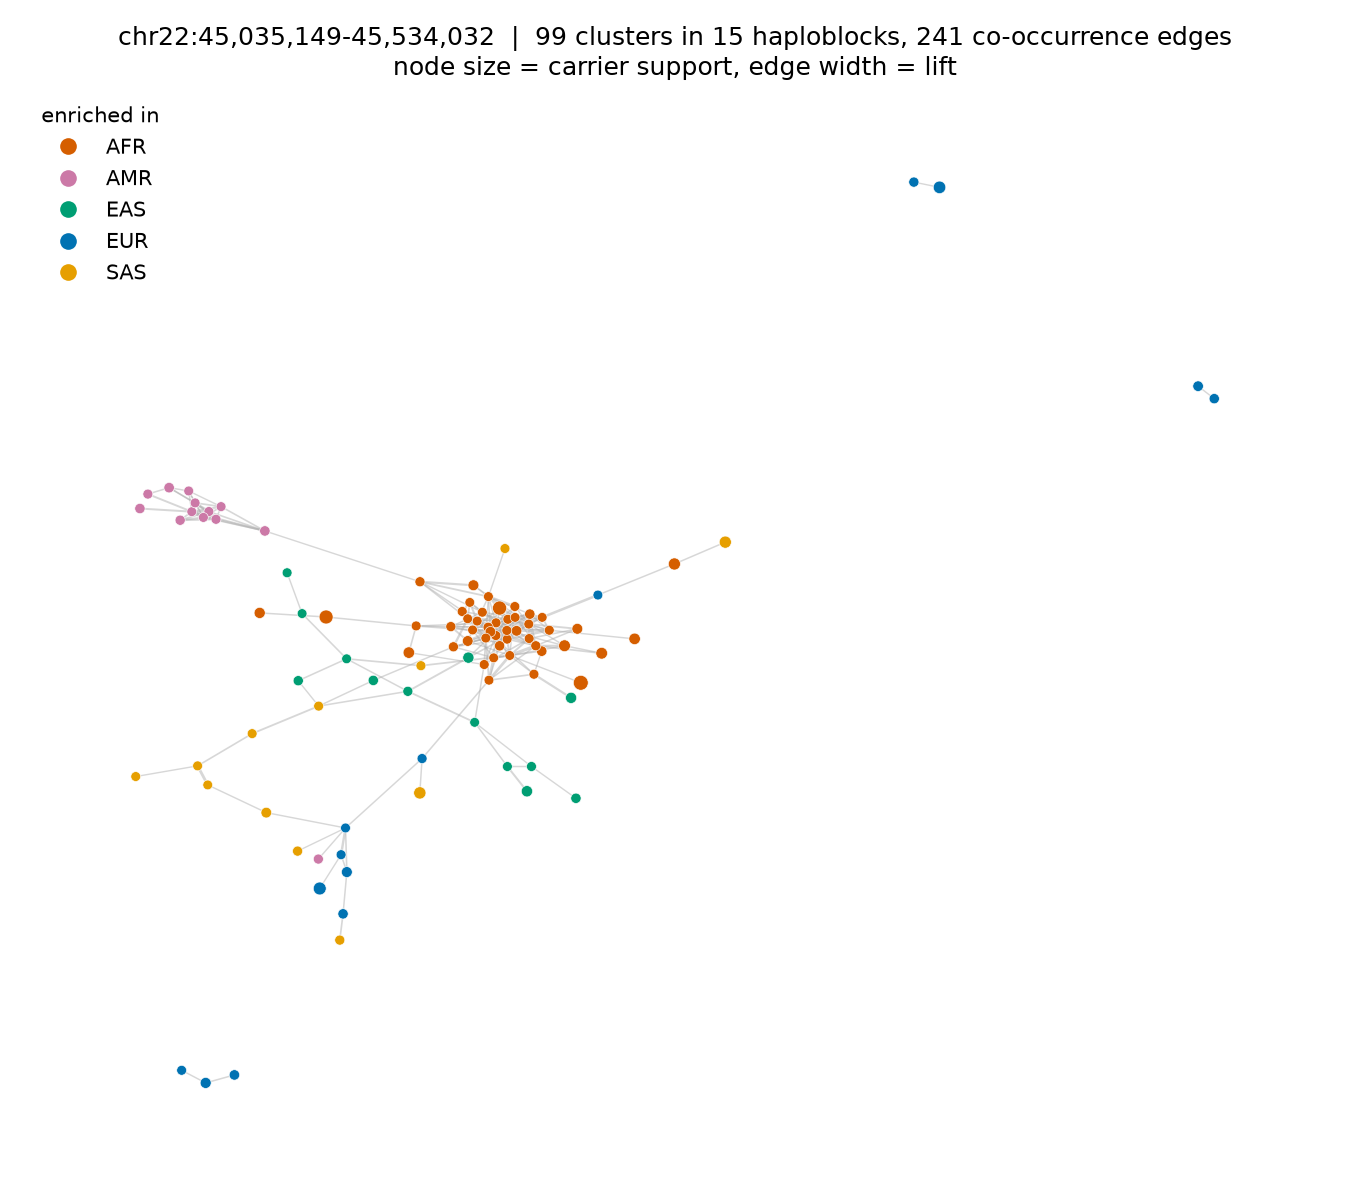
\includegraphics[width=0.80\linewidth]{graph_region.png}
\caption{One region of chr22 (the densest published island): clusters as nodes coloured by the ancestry they are enriched in, co-occurrence edges weighted by lift.}
\end{figure}

\begin{figure}[htbp]
\centering
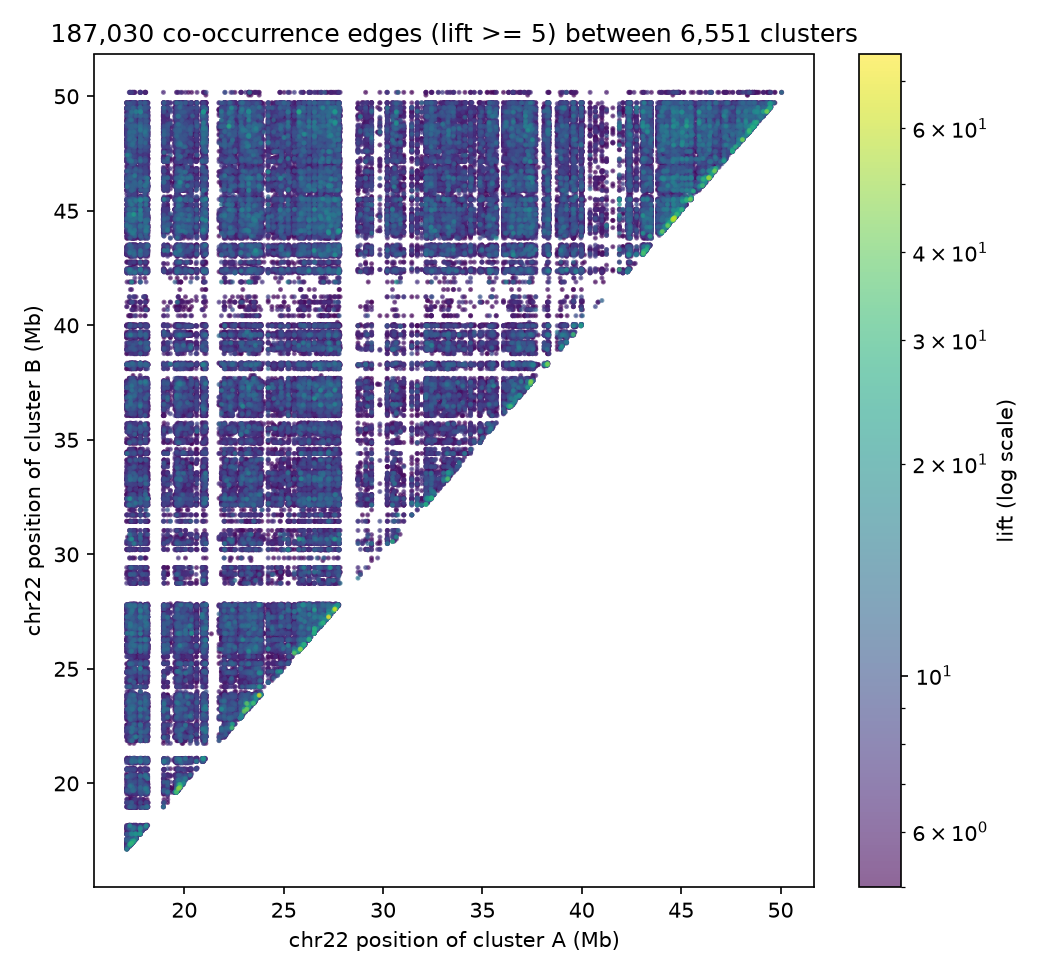
\includegraphics[width=0.70\linewidth]{graph_edge_positions.png}
\caption{All 187,030 co-occurrence edges plotted by the positions of their two endpoints: block structure and long-range population structure.}
\end{figure}

\begin{figure}[htbp]
\centering
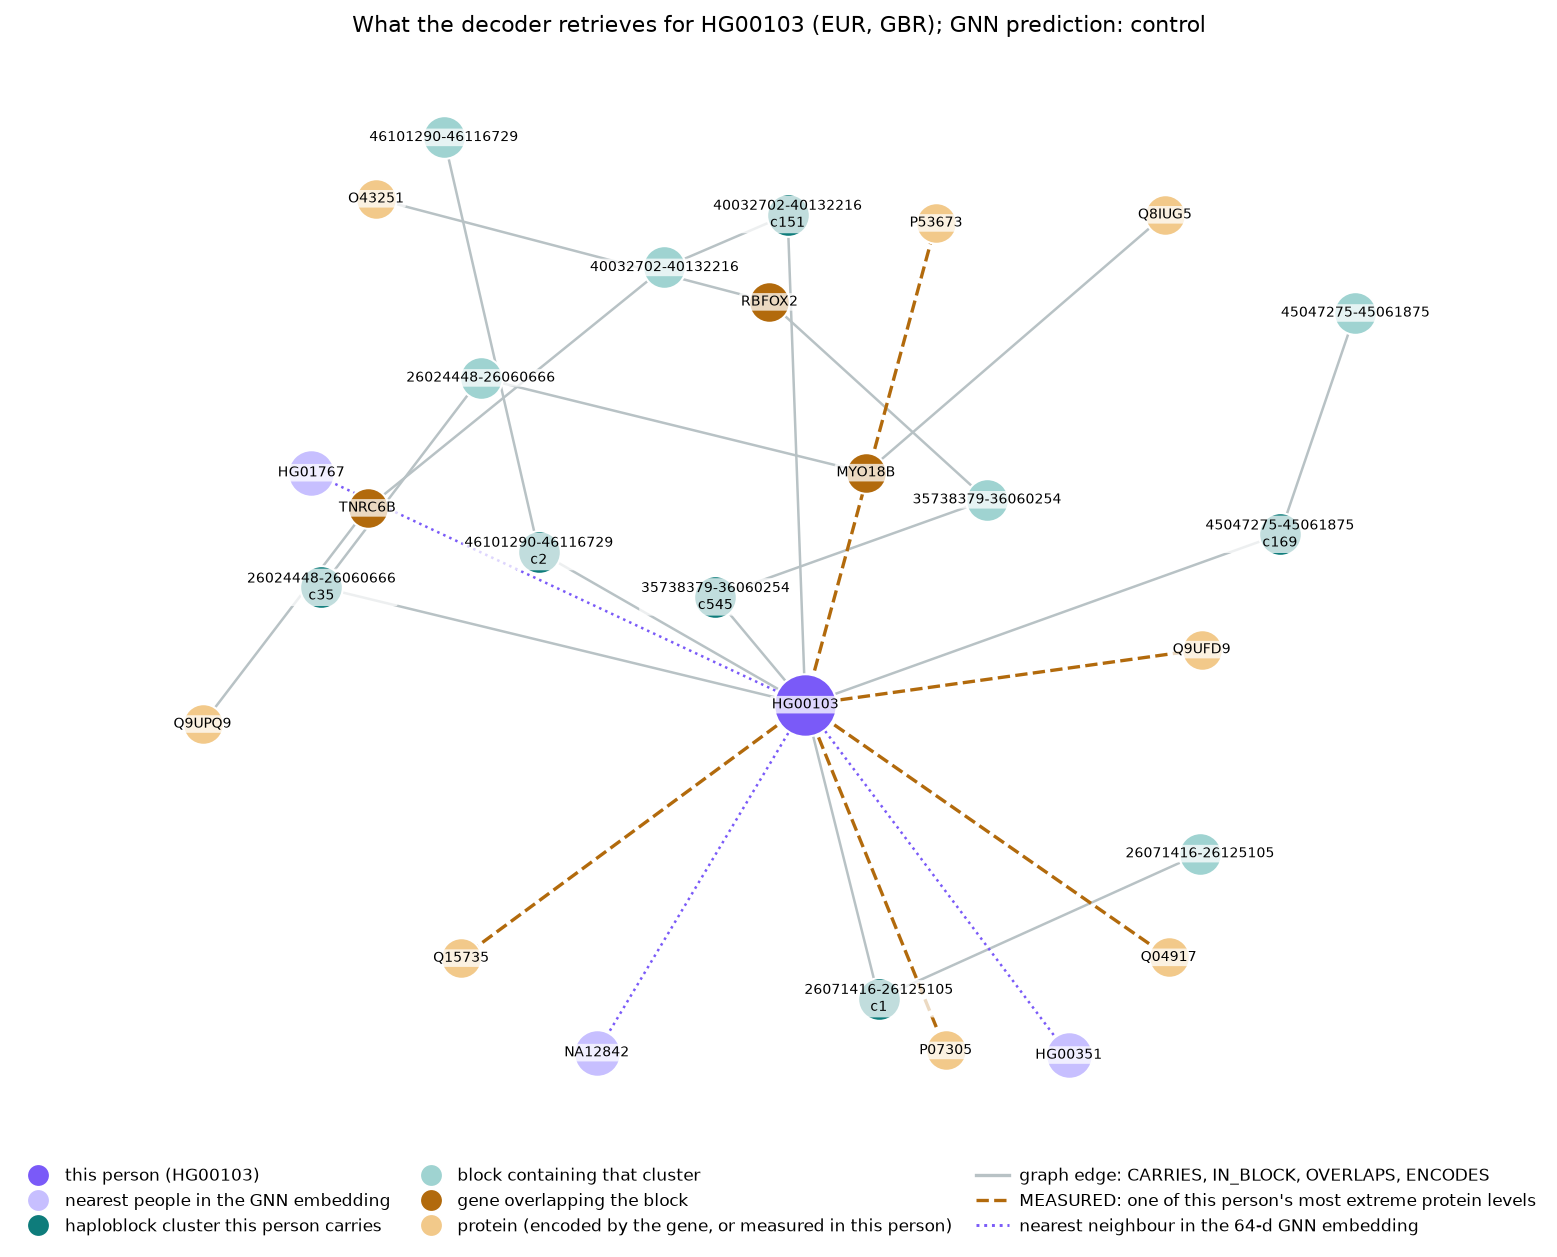
\includegraphics[width=0.85\linewidth]{person_neighbourhood.png}
\caption{A real person's neighbourhood in the graph (HG00103), as the decoder retrieves it: clusters, blocks, genes, proteins, extreme protein levels and nearest neighbours in the embedding.}
\end{figure}

\subsection{7. From graph to embeddings}

A GNN needs a starting vector for every node. Cluster and block nodes use their statistics (support, block length, entropy, dominance, and so on), standardised. People and clusters together get a truncated singular value decomposition of the carrier matrix M (2,548 x 6,551): M is approximated as U S V-transpose with 32 components; the rows of U S are 32-number vectors for people and the rows of V S are 32-number vectors for clusters, in one shared space, so a person sits near the clusters they carry and near people with similar haplotypes. No labels are used, so nothing can leak into the test set. Alternatives implemented and compared: Node2Vec random-walk embeddings on the person-cluster graph (GPU, via pyg-lib; with 50 pretraining epochs it reaches 0.950 on ancestry against 0.974 for SVD, with the same 0.70 silhouette), free learned embeddings (0.585), and the raw 6,551-long carrier row.

Where the phenotypes enter: only as training targets. The GNN is trained to predict the label from a person's neighbourhood; the loss reshapes all weights so the learned 64-number vectors separate the phenotype groups. The quality of a space is measured by the silhouette score (how compact and separated the groups are) and by a 5-nearest-neighbour classifier: plain SVD scores silhouette 0.06 and 5-NN accuracy 0.90 by ancestry; the GNN's hidden layer scores 0.70 and 0.97. That 0.06 to 0.70 is the GNN's contribution. With free learned embeddings instead of SVD initialisation the GNN reaches only 0.585 balanced accuracy on ancestry: the starting embedding matters more than the architecture.

\begin{figure}[htbp]
\centering
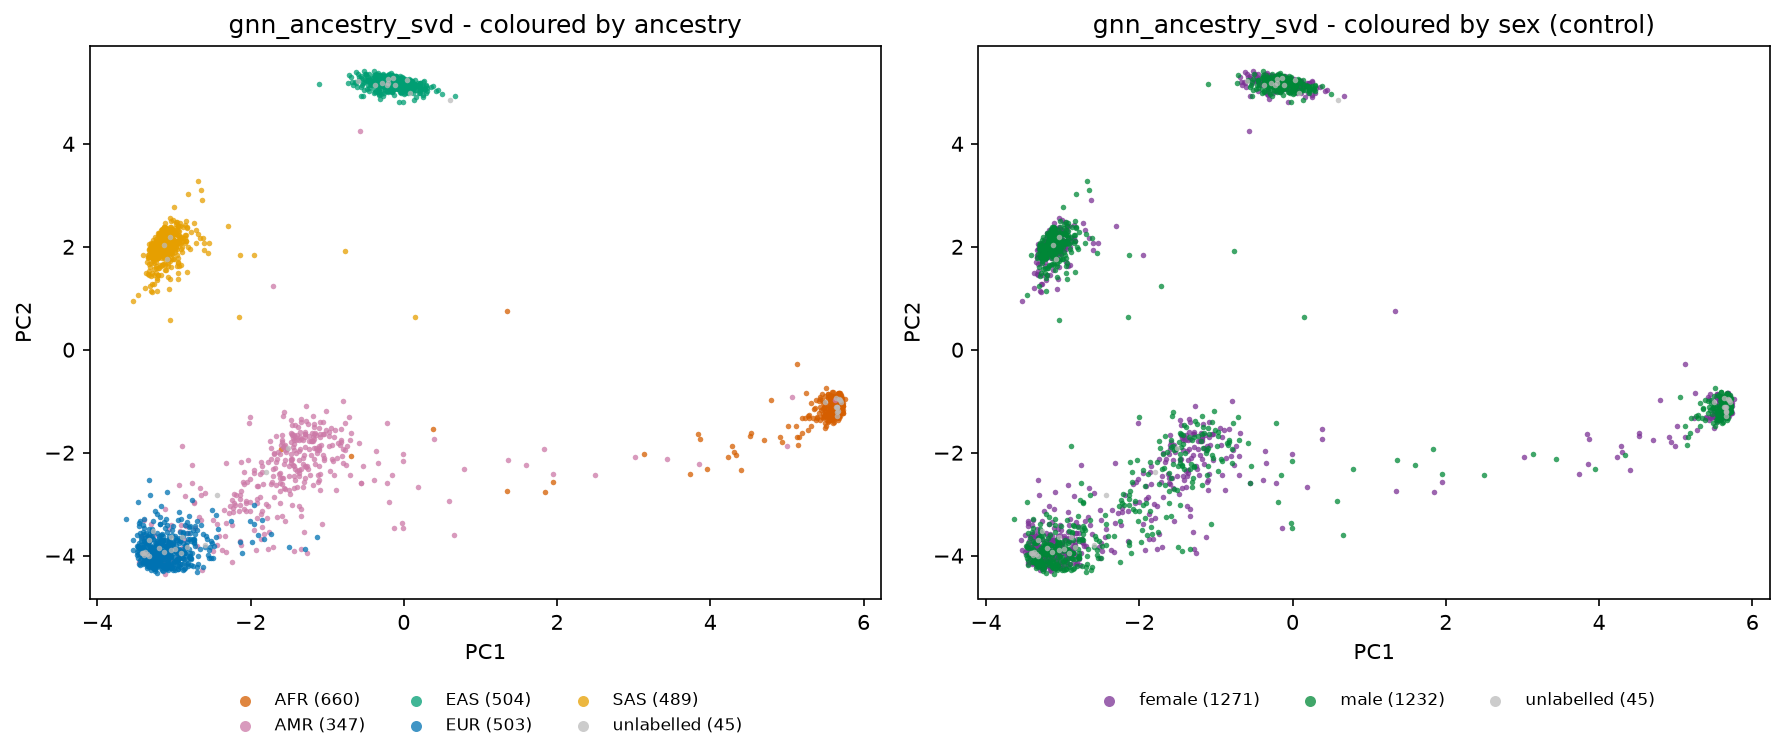
\includegraphics[width=0.95\linewidth]{embedding_individuals.png}
\caption{The GNN's 64-dimensional embedding of people projected to two dimensions: five ancestry groups separate cleanly (AMR spread between EUR and AFR, as admixture predicts); coloured by sex the same points are fully mixed.}
\end{figure}

\begin{figure}[htbp]
\centering
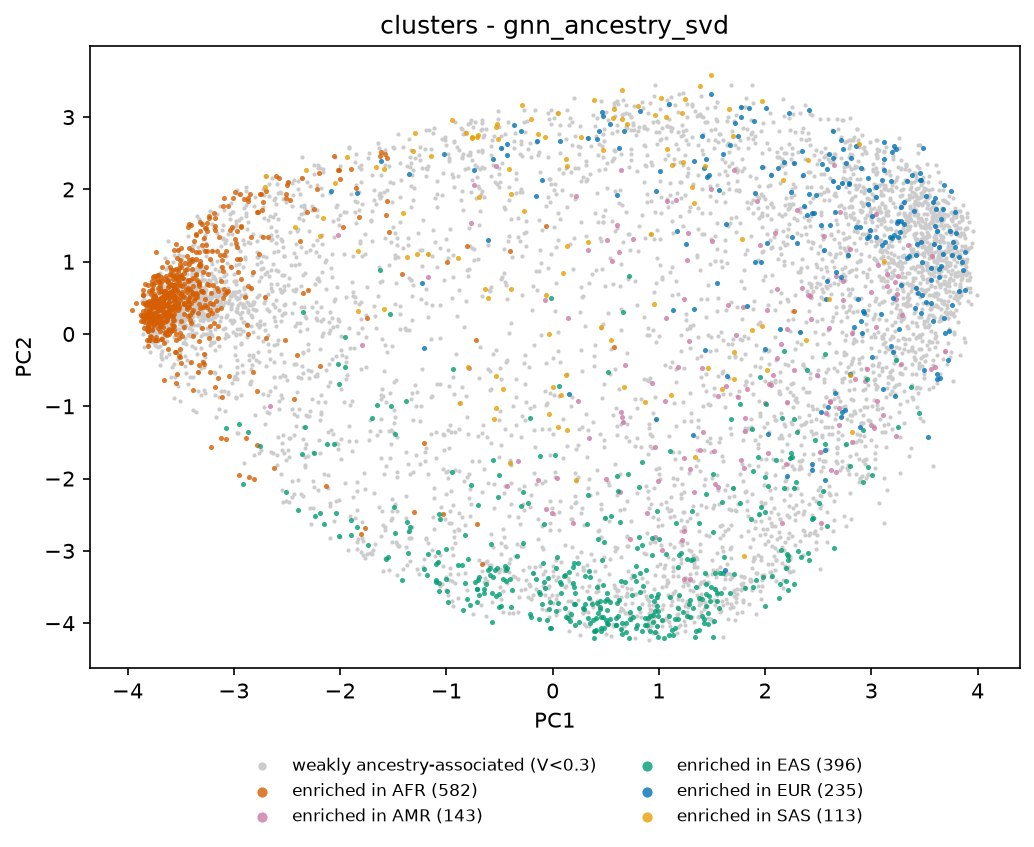
\includegraphics[width=0.70\linewidth]{embedding_clusters.png}
\caption{The same model's embedding of clusters, coloured by the ancestry each cluster is enriched in.}
\end{figure}

\begin{figure}[htbp]
\centering
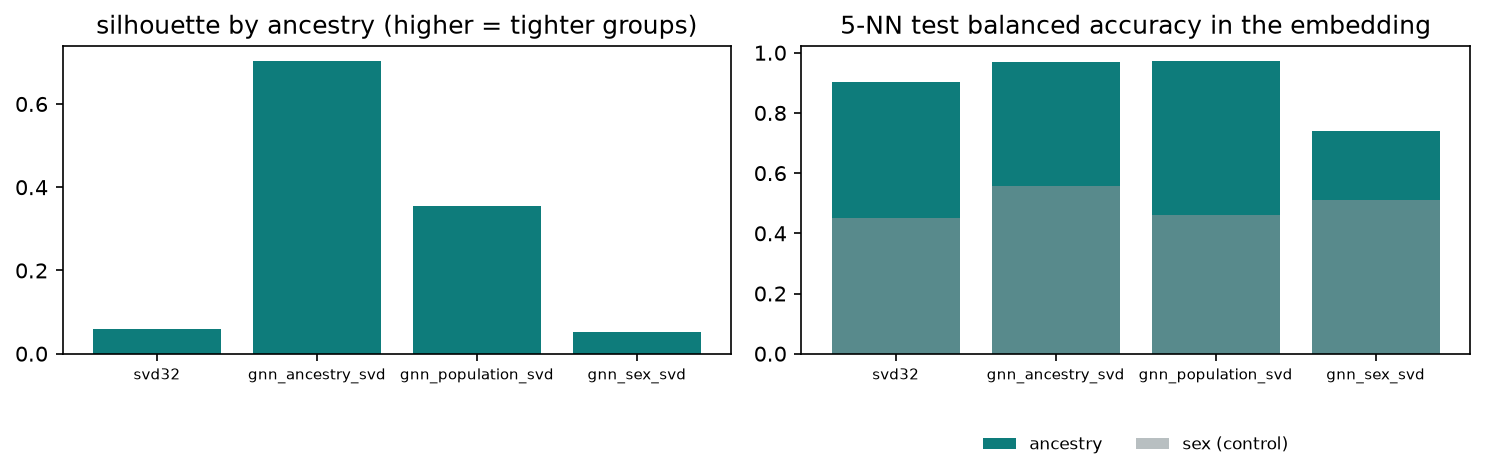
\includegraphics[width=0.90\linewidth]{embedding_quality.png}
\caption{Embedding quality: silhouette by ancestry and 5-nearest-neighbour accuracy for SVD and for each GNN's hidden layer; sex stays at chance.}
\end{figure}

\begin{figure}[htbp]
\centering
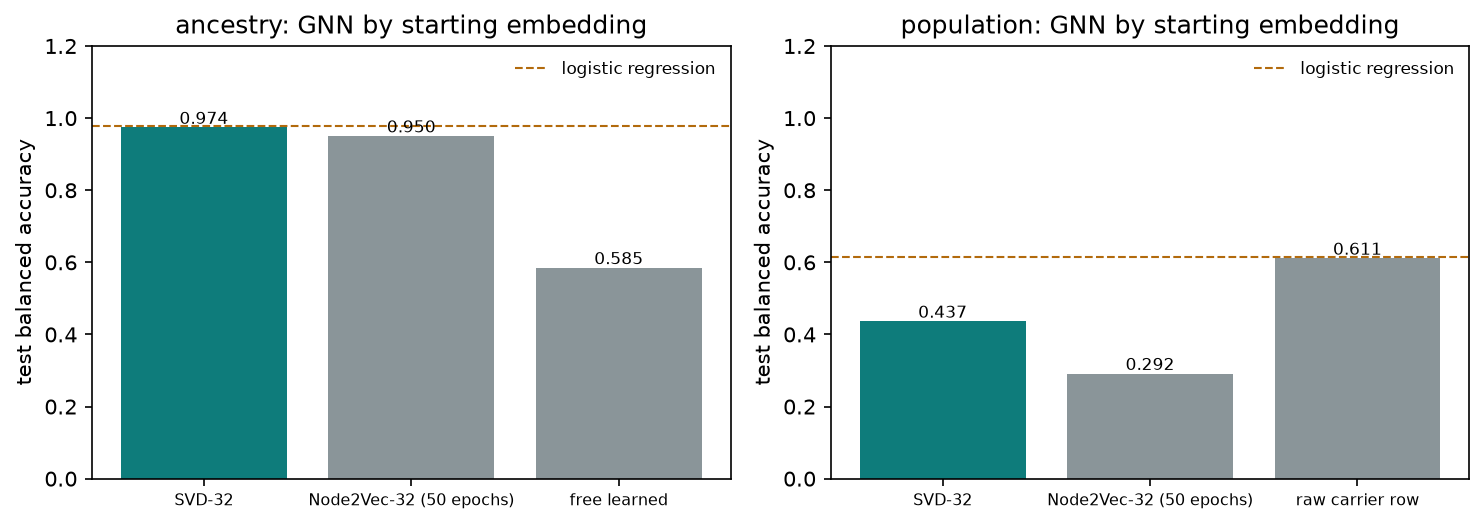
\includegraphics[width=0.90\linewidth]{init_comparison.png}
\caption{The same GNN with different starting embeddings for the person nodes: SVD-32, Node2Vec-32 (50 pretraining epochs, A100), free learned embeddings and the raw carrier row, against the logistic-regression line.}
\end{figure}

\subsection{8. The encoder: a heterogeneous graph neural network}

Architecture (PyTorch Geometric HeteroConv, two layers, hidden size 64): a linear projection per node type to 64 numbers; then two rounds of message passing in which, for every relation, SAGEConv adds the mean of a node's neighbours to its own state (carries, in\_block, next\_block, overlaps, encodes, each in both directions) and GraphConv adds an edge-weighted mean for co\_occurs (weight = normalised log lift) and measured (weight = the protein's harmonised z-score, signed, so a high protein pushes positively and a low one negatively); after each round LayerNorm, a residual connection, ReLU and dropout 0.3; a linear head from the person's 64 numbers to class scores. After round one a person has absorbed their clusters (and proteins); after round two, what those clusters co-occur with, their blocks, and the genes and proteins in those blocks.

Training: class-weighted cross-entropy on training people only (weights inversely proportional to class size so AMR and small populations count); Adam with learning rate 0.005 and weight decay 0.0005; early stopping on validation balanced accuracy with patience 30, best weights restored. Full-batch: one epoch is one pass over the whole graph (about 2.4 million CARRIES, 0.37 million CO\_OCCURS and 1.07 million MEASURED edges), 0.95 s on an M2 laptop CPU and 0.10 s on an A100 GPU. About 105 thousand parameters with SVD input, about 500 thousand with the raw carrier row.

\begin{longtable}{p{0.282\linewidth}p{0.141\linewidth}p{0.235\linewidth}p{0.282\linewidth}}
\toprule
\textbf{Target (real labels)} & \textbf{Classes} & \textbf{Logistic regression} & \textbf{GNN} \\
\midrule
\endhead
ancestry & 5 & 0.977 & 0.974 (SVD input) \\
population & 26 & 0.614 & 0.611 (raw input; 0.437 with SVD-32) \\
sex (negative control) & 2 & 0.463 & 0.503 \\
\bottomrule
\end{longtable}

Reading: balanced accuracy on the held-out 376 people. On chr22 alone ancestry and population are almost linear functions of which clusters a person carries, so the GNN ties the linear baseline on accuracy; it wins on the embedding space and, as the next section shows, on integration.

\subsubsection{Metrics, defined}

\begin{itemize}[leftmargin=1.4em]
  \item Accuracy: correct predictions divided by all predictions. Misleading when classes are unequal (predicting control for everyone scores 64\% on the phenotype).
  \item Balanced accuracy: the mean over classes of the recall of that class (correct in class k divided by the number truly in class k). Chance is 1/k: 0.20 for ancestry, 0.038 for population, 0.5 for sex, 0.33 for site.
  \item Macro-F1: for each class the harmonic mean of precision and recall, averaged over classes.
  \item ROC-AUC: the probability that a randomly chosen case receives a higher case score than a randomly chosen control; 0.5 is chance, 1.0 is a perfect ranking. Only defined for two classes.
  \item R-squared per protein: 1 minus the residual sum of squares divided by the total sum of squares, on test people with an observed value (at least five); negative means worse than predicting the mean.
  \item Silhouette: for each person, the mean distance to their own group minus the mean distance to the nearest other group, scaled to -1..1; averaged. Higher means tighter, better separated groups in the embedding.
  \item 5-nearest-neighbour accuracy: label a test person by majority vote of the five nearest training people in the embedding; balanced accuracy of that vote.
  \item Precision at 20: of the twenty clusters with the highest saliency, the fraction that are planted causal clusters; chance is 20 / 6,551 x 20 = 0.06.
  \item Cramer's V: sqrt(chi-square / N) for a 2 x k table; 0 means the cluster is independent of the label, 1 means it determines it.
  \item Early stopping and model selection use the validation people only; every number reported in this document is on the test people.
\end{itemize}

\begin{figure}[htbp]
\centering
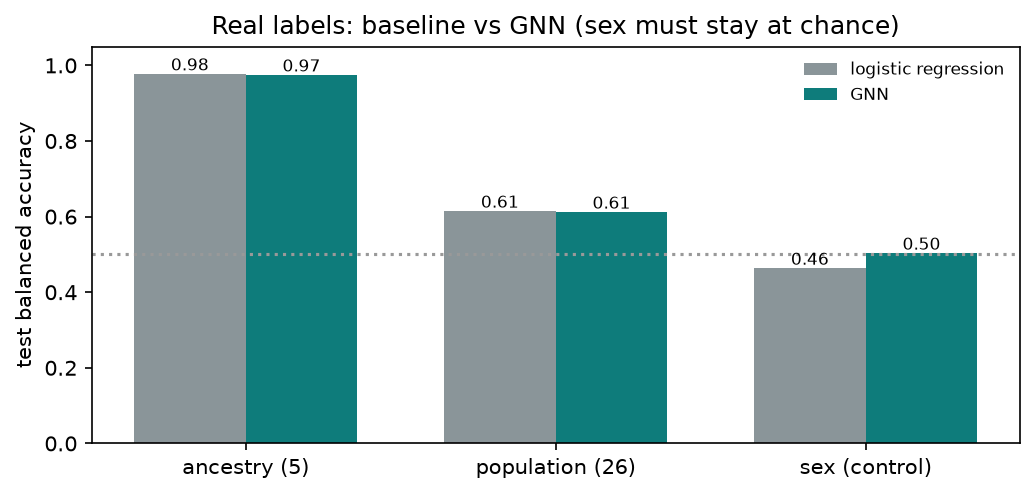
\includegraphics[width=0.70\linewidth]{baseline_vs_gnn.png}
\caption{Real labels: logistic regression versus the GNN; sex, the negative control, stays at chance for both.}
\end{figure}

\subsection{9. Integrating the proteome (schema v2)}

The synthetic proteome we generated is keyed to the real 1000G ids and has a saved ground truth (ground\_truth.json). Per person: a site assigned at random within each ancestry (so site is a pure batch effect), the real sex, a random age; a case/control phenotype whose log-odds is a weighted sum over 20 causal haploblock clusters plus a small age term, calibrated to 38\% cases; each causal cluster also shifts one protein encoded in its own block (a cis effect); 15\% of proteins respond to the phenotype, all respond to age and sex; a per-site batch shift; and missingness that increases toward the detection limit. The first version shifted every protein with the phenotype and every model scored 1.0, the same trap an earlier team result fell into, so the signal was made sparse.

Before entering the graph, protein levels pass a harmoniser: within each site and protein, z = (value - median) / (1.4826 x median absolute deviation). Computed from each site's own samples, it removes the between-site shift completely (0.48 to 0.00 log2) while 227 proteins keep their phenotype association. Missing values stay missing; they simply create no MEASURED edge and are never imputed as zero.

\begin{longtable}{p{0.263\linewidth}p{0.254\linewidth}p{0.188\linewidth}p{0.094\linewidth}p{0.141\linewidth}}
\toprule
\textbf{Model} & \textbf{Input to the person node} & \textbf{Graph relations} & \textbf{AUC} & \textbf{Balanced accuracy} \\
\midrule
\endhead
genome only & SVD-32 or raw carrier row & genome relations & 0.60-0.63 & 0.57-0.62 \\
proteome only (MLP, no graph) & harmonised z + observed mask (920 numbers) & none & 0.96 & 0.96 \\
genome + proteome (graph) & both & all twelve relations & 0.99 & 0.97 \\
site (batch control, full graph) & both & all & - & 0.30 (chance 0.33) \\
ancestry (full graph) & both & all & - & 0.90 \\
\bottomrule
\end{longtable}

The graph adds signal on top of the proteome, and the site control shows none of it is batch. A gradient saliency on the raw carrier input ranks clusters by their influence on the case score: 3-4 of the top 20 are ground-truth causal clusters (1.2 expected by chance). One negative result is kept deliberately: predicting the proteome from the genome embedding gives R-squared near zero even for cis-affected proteins, whereas a per-protein ridge regression on the carrier row recovers the strong cis effects (4 of 20 cis proteins with test R-squared above 0.1, 0 of 440 others). The GNN is the integration and embedding tool; discovering single-cluster cis effects needs sparse per-protein models or a prior from published protein-QTL data.

\begin{figure}[htbp]
\centering
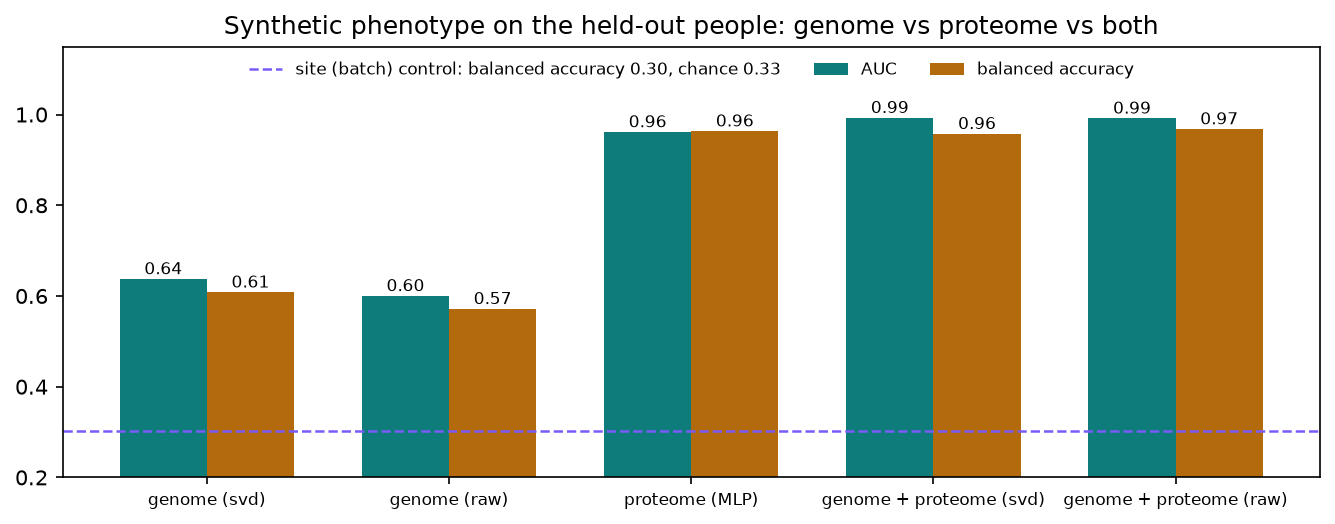
\includegraphics[width=0.90\linewidth]{results_modalities.png}
\caption{Held-out AUC and balanced accuracy for the synthetic phenotype by modality; the site control sits at chance.}
\end{figure}

\begin{figure}[htbp]
\centering
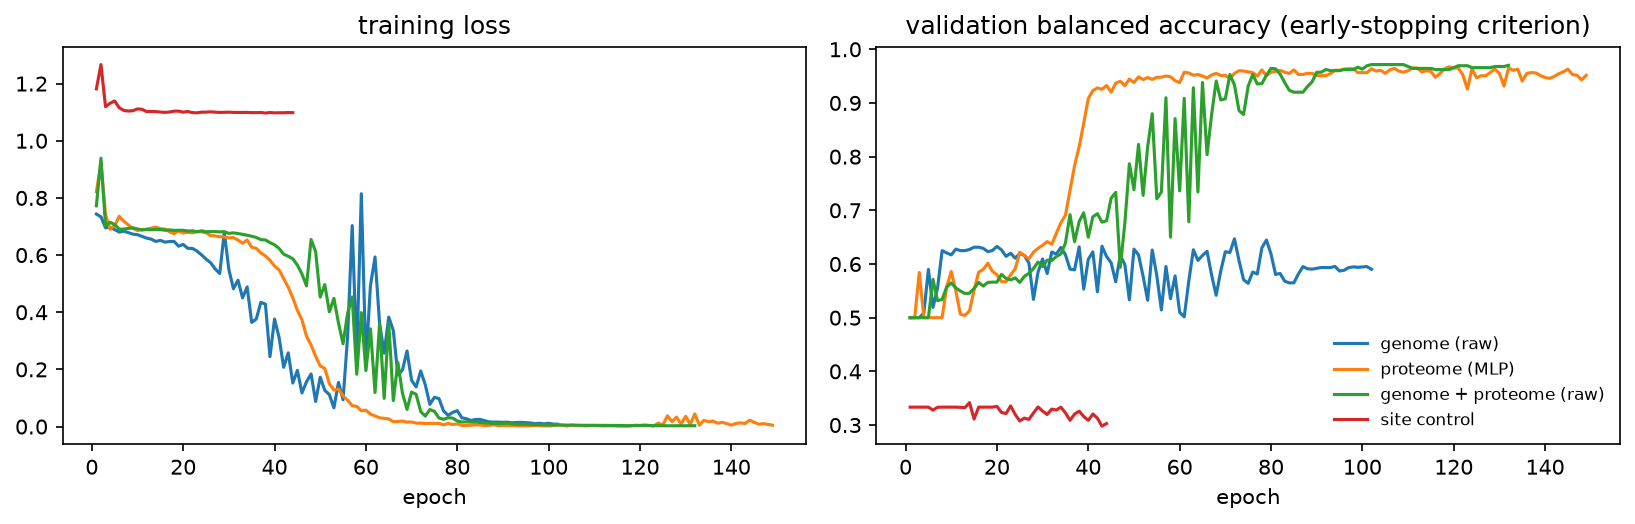
\includegraphics[width=0.95\linewidth]{training_curves.png}
\caption{Training loss and validation balanced accuracy per epoch for the v2 runs (early stopping picks the best validation epoch).}
\end{figure}

\begin{figure}[htbp]
\centering
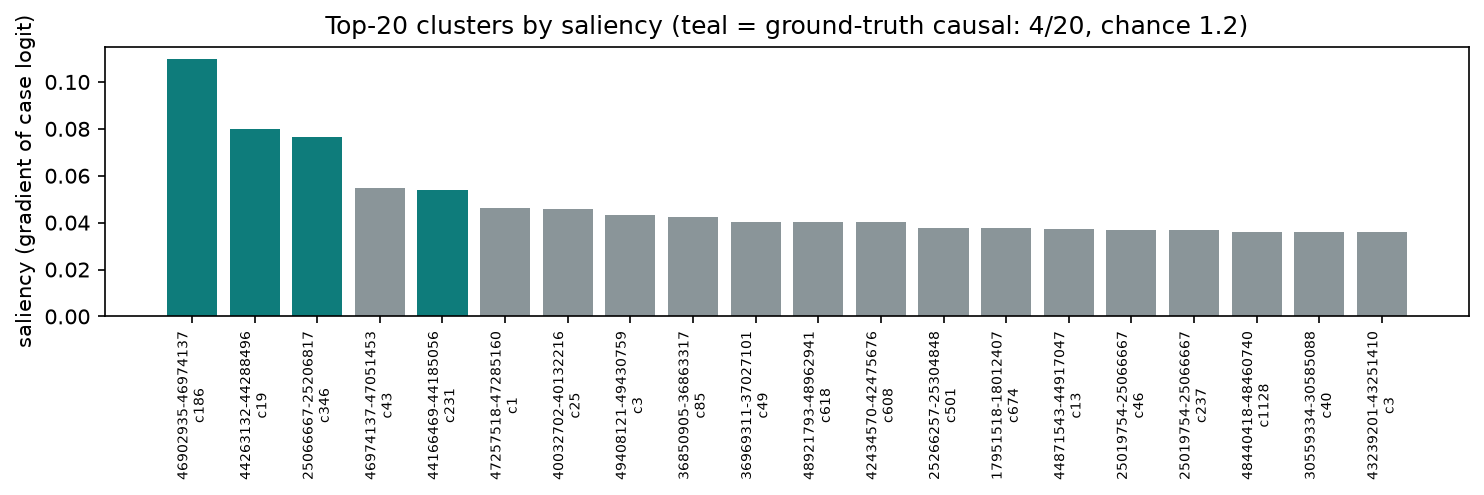
\includegraphics[width=0.95\linewidth]{saliency_top20.png}
\caption{Cluster saliency of the combined model: ground-truth causal clusters (teal) among the top 20.}
\end{figure}

\begin{figure}[htbp]
\centering
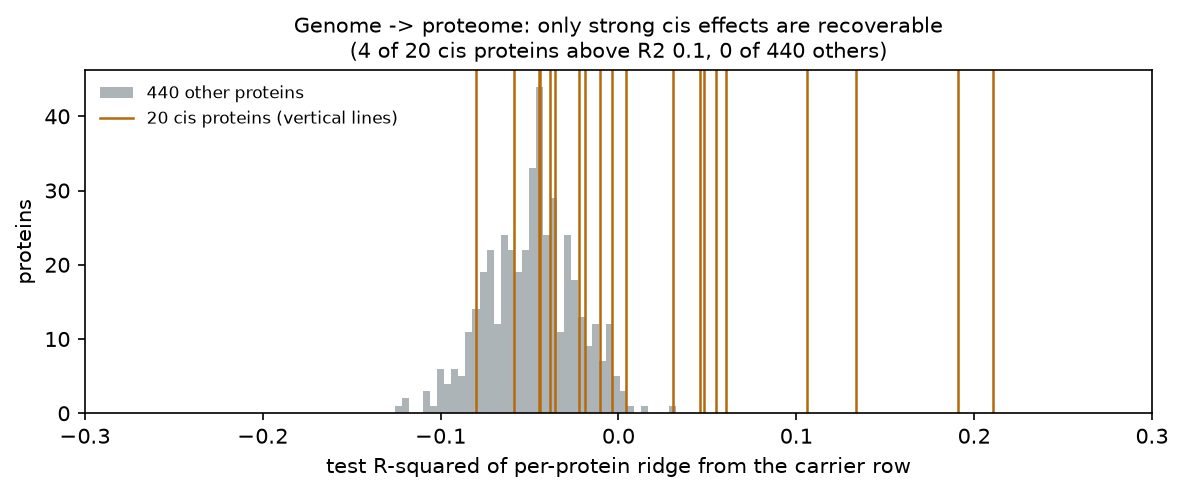
\includegraphics[width=0.85\linewidth]{ridge_r2.png}
\caption{Per-protein ridge from the genome: only the strong cis effects are recoverable.}
\end{figure}

\subsection{10. The decoder: GraphRAG with an NVIDIA NIM language model}

For one person the decoder retrieves, deterministically and only from the graph: the profile (ancestry, population, sex, site, age; the true phenotype withheld), the GNN's prediction, the globally salient clusters the person carries, their eight most ancestry-informative clusters with block, genes and proteins, their eight most extreme protein levels with the encoding block and whether that block holds a notable cluster, and their five nearest people in the GNN embedding. This is serialised as JSON (about 4,500 tokens) and sent to nvidia/nemotron-3-super-120b-a12b through NVIDIA's OpenAI-compatible NIM endpoint with reasoning\_effort set to none (otherwise this reasoning model thinks inline and exhausts the token budget before answering) under a system prompt that forbids inventing entities and requires every id to be cited verbatim. The reply's cited ids are checked against the context before anything is written. For person HG00103 the model answered in 13 seconds with 25 cited ids and none unknown, producing a summary, ancestry and phenotype assessments, genome-proteome links (for example cluster chr22\_40032702-40132216\_cluster151 in the block encoding TNRC6B / Q9UPQ9) and caveats stating that the phenotype is synthetic and ancestry is population structure, not a medical finding.

\subsection{11. Federated learning with NVFlare}

\begin{figure}[htbp]
\centering
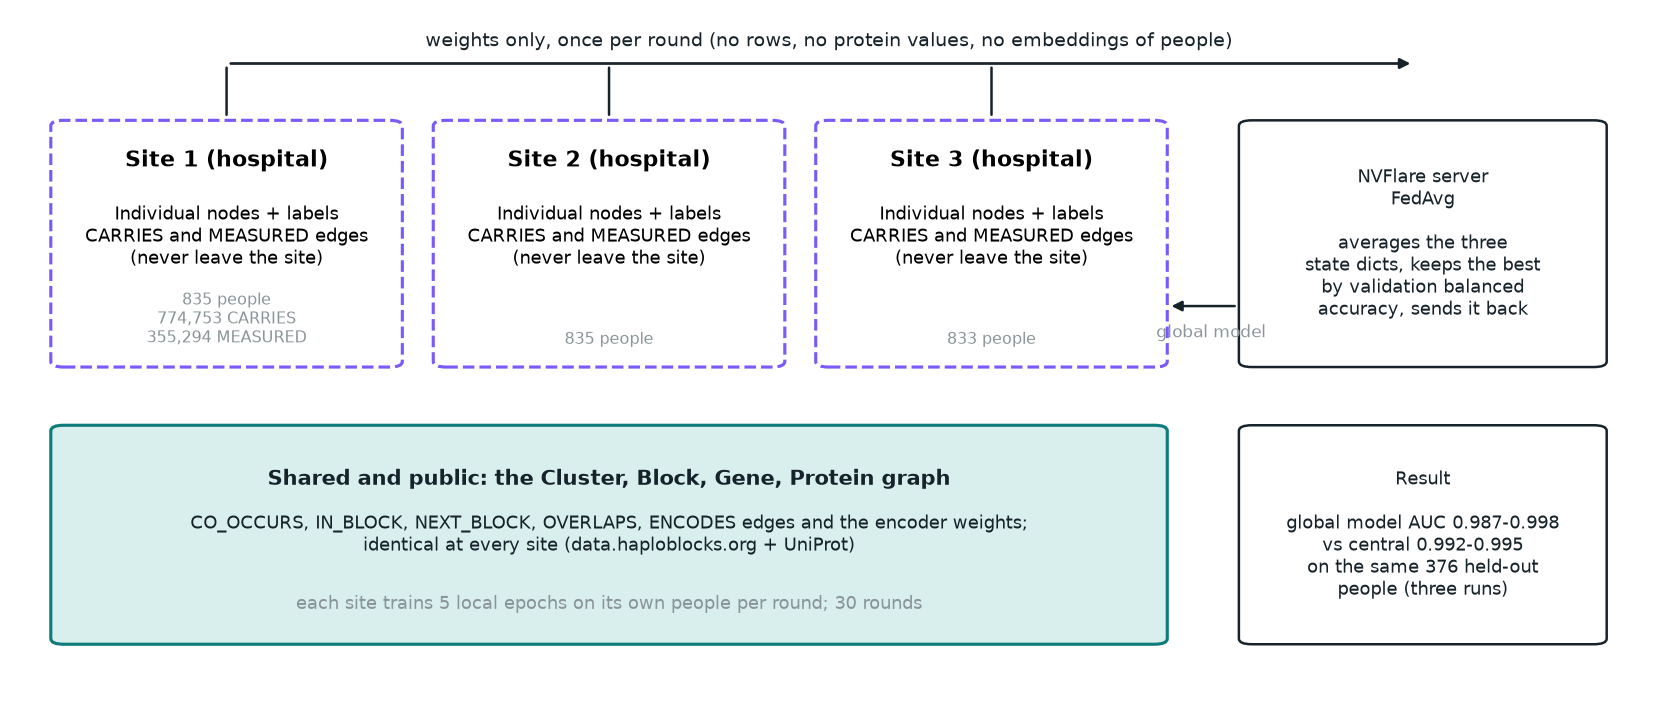
\includegraphics[width=0.95\linewidth]{federated_topology.png}
\caption{Federated topology: three sites with private people and edges, one shared public graph, weights only to the server.}
\end{figure}

Partition: site s receives the people whose site code is s (835 / 835 / 833, mixed ancestry). Its graph is PyG's HeteroData.subgraph restricted to those people: their nodes are re-indexed, their CARRIES and MEASURED edges kept, and every other node type and edge kept whole because those are public. Site 1, for instance, holds 835 people, 774,753 CARRIES and 355,294 MEASURED edges. The person's input (carrier row plus harmonised protein vector and mask) is computed from the site's own rows; no cross-site preprocessing exists because the harmoniser is already per site.

Mechanics (NVFlare 2.9, FedAvgRecipe with the PyTorch Client API): job.py derives every model constructor value from the public graph into model\_args.json so the server and all clients build byte-identical models. Each client runs flare.init(), builds its site graph once, then loops: receive the global weights, evaluate them on its own validation and test people, train five full-batch epochs on its own training people, send back the weights, the metrics and the number of optimizer steps. The server averages the weights (weighted by steps, equal here) and selects the best global model by validation balanced accuracy. What crosses the site boundary per round: one state dict of about half a million numbers and five scalars; no rows, no protein values, no embeddings of people.

\begin{longtable}{p{0.376\linewidth}p{0.188\linewidth}p{0.141\linewidth}p{0.235\linewidth}}
\toprule
\textbf{Model} & \textbf{Balanced accuracy} & \textbf{AUC} & \textbf{Evaluated on} \\
\midrule
\endhead
federated global model, 10 rounds x 5 epochs & 0.90 & 0.955 & the same 376 held-out people \\
federated global model, 30 rounds x 5 epochs & 0.963 & 0.998 & the same 376 held-out people \\
central model (train\_gnn\_v2, both/raw) & 0.969 & 0.992 & the same 376 held-out people \\
federated model per site (30 rounds) & 0.983 / 0.981 / 0.933 & 1.000 / 0.999 / 0.997 & each site's own held-out people \\
\bottomrule
\end{longtable}

\begin{figure}[htbp]
\centering
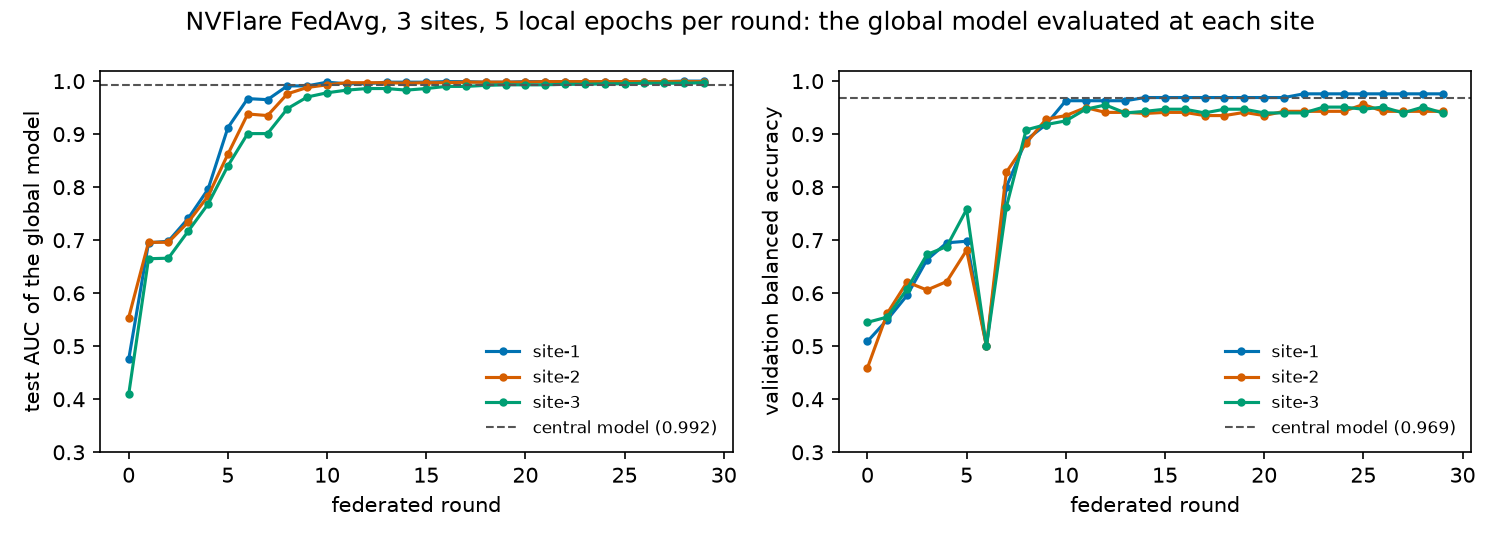
\includegraphics[width=0.95\linewidth]{federated_rounds.png}
\caption{FedAvg convergence: the global model's AUC and validation balanced accuracy at each site, per round, against the central model.}
\end{figure}

\begin{figure}[htbp]
\centering
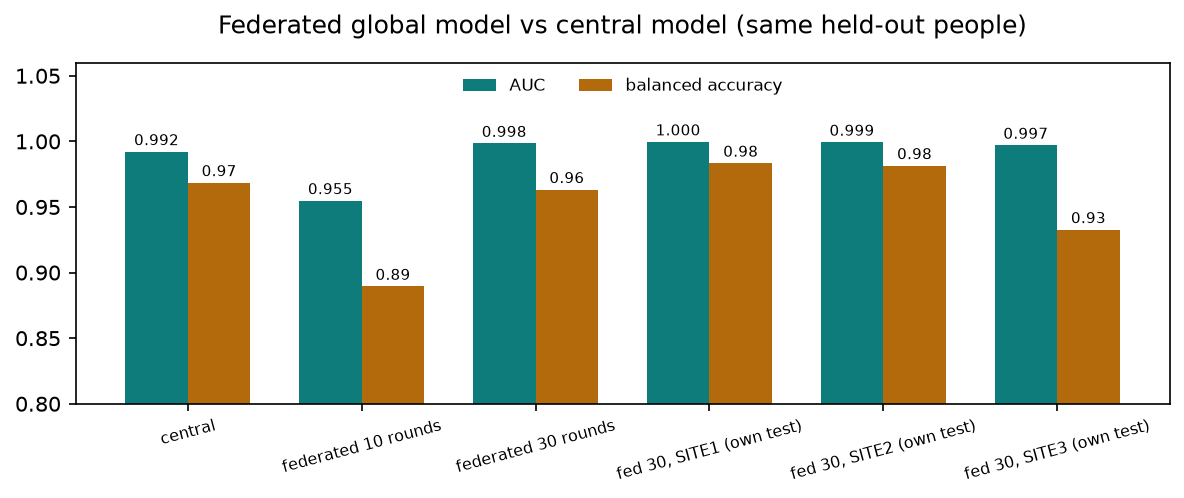
\includegraphics[width=0.90\linewidth]{federated_vs_central.png}
\caption{Central versus federated (10 and 30 rounds) on the same held-out people, and the federated model on each site's own held-out people.}
\end{figure}

Ten rounds (50 local steps) were short of the central run's \textasciitilde{}80 epochs; thirty rounds converge to the central model's level. Federated training loses nothing here because the sites are random draws of the same population by construction; with ancestry-pure sites the averaging would have to fight client drift, which is the next experiment.

\subsubsection{With and without federation, on this data}

federated/local\_only.py trains each site alone on its own people for the same 150 optimizer steps the federated clients used, then scores that lone model on its own held-out people and on the other sites' held-out people. On this synthetic data a lone site already does well, because 835 people and a strong proteome signal are enough: own-site AUC SITE1 0.998, SITE2 0.986, SITE3 0.988; the worst transfer of a lone model to another site's people is SITE1 0.949, SITE2 0.969, SITE3 0.997. The federated global model scores SITE1 0.999, SITE2 1.000, SITE3 0.968 on the same per-site people and 0.987 to 0.998 on the pooled held-out set across runs. With a smaller budget the picture changes: at 50 optimizer steps per site (a 10-round run inside the Docker image on the A100) a lone site reaches only 0.88 to 0.92 while the federated model reaches 0.989 to 0.998 on the same per-site people, because the averaged weights have effectively seen every site's people. So federation costs nothing when a site has enough data and budget and helps clearly when it does not; in both cases what it solves is the constraint, not the score: one shared model, trained on everyone, with no row leaving any site. A larger gain is expected when sites differ systematically (ancestry-pure hospitals, different protein panels), which is the ancestry-partitioned experiment listed under next steps.

\begin{figure}[htbp]
\centering
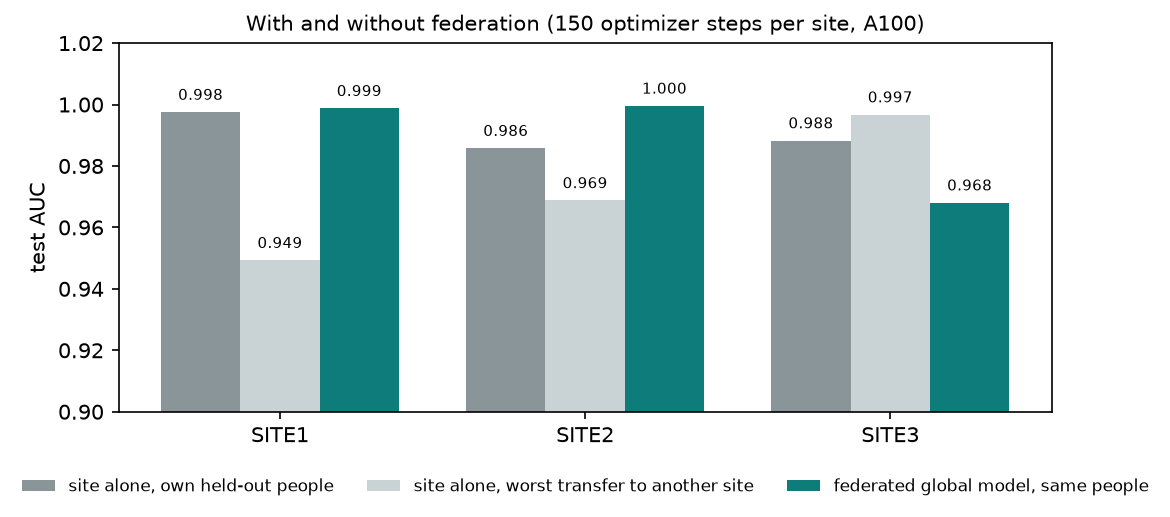
\includegraphics[width=0.80\linewidth]{federated_site_alone.png}
\caption{With and without federation: each site trained alone on its own people versus the federated global model, scored on the same held-out people per site (A100 re-run).}
\end{figure}

\begin{longtable}{p{0.301\linewidth}p{0.160\linewidth}p{0.160\linewidth}p{0.160\linewidth}p{0.160\linewidth}}
\toprule
\textbf{Site (held-out n)} & \textbf{Alone, 150 steps} & \textbf{Federated, 150 steps} & \textbf{Alone, 50 steps} & \textbf{Federated, 50 steps} \\
\midrule
\endhead
SITE1 (111) & 0.998 / 0.952 & 0.999 / 0.983 & 0.881 / 0.543 & 0.998 / 0.950 \\
SITE2 (136) & 0.986 / 0.852 & 1.000 / 0.991 & 0.902 / 0.772 & 0.991 / 0.907 \\
SITE3 (129) & 0.988 / 0.923 & 0.968 / 0.933 & 0.915 / 0.830 & 0.989 / 0.865 \\
average over sites & 0.991 / 0.909 & 0.989 / 0.969 & 0.899 / 0.715 & 0.993 / 0.907 \\
pooled 376 people, federated global model & - & 0.987 / 0.967 & - & 0.991 / 0.901 \\
pooled 376 people, central model & 0.995 / 0.960 &  & 0.997 / 0.959 &  \\
\bottomrule
\end{longtable}

AUC / balanced accuracy on each site's own held-out people. Transfer of a lone model to other sites' people (150 steps, AUC): the SITE1 model scores 0.982 on SITE2 people and 0.949 on SITE3 people; SITE2: 0.993 and 0.969; SITE3: 0.997 and 0.998; the federated model 0.999 / 1.000 / 0.968 on the three sites.

\subsubsection{Why federated, and what kind}

The mission sentence of the README is a statement about where data lives: a hospital may compute on its patients but may not ship their rows. This is horizontal federated learning: every site has the same columns (the same graph schema, the same protein panel) and different rows (different people). It is not a split of the genome across sites (each site would then hold part of every person, which is vertical federation and a different problem) and not a way to add chromosomes: another chromosome is another shared reference graph, added at every site at once. What is gained is the ability to train on all 2,503 people while each site only ever reads its 835; what is lost, in this experiment, is nothing measurable, because the sites are alike. A real deployment would report each site's own held-out score and never assemble a central test set.

\subsubsection{Mechanics in detail}

\begin{itemize}[leftmargin=1.4em]
  \item Model definition (federated/model.py): the same architecture as train\_gnn\_v2, copied into a self-contained file so the NVFlare server can import it without the pipeline. Its constructor reads model\_args.json (input sizes per node type, the twelve relations, hidden 64, two layers, dropout 0.3, mean aggregation) so server and clients build identical state dicts.
  \item Job (federated/job.py): FedAvgRecipe(name, model class path and args, min\_clients 3, num\_rounds, train\_script client.py, train\_args, key\_metric val\_balanced\_accuracy, server\_expected\_format PYTORCH); add\_decomposers registers TensorDecomposer so tensors travel natively; add\_server\_file ships model.py to the server; SimEnv(num\_clients 3, workspace\_root) runs the three sites as threads on one machine; recipe.execute(env) writes the job and runs it.
  \item Client (federated/client.py): flare.init(); the site name (site-1, site-2, site-3) selects the site code; HeteroData.subgraph keeps that site's people and their CARRIES and MEASURED edges and leaves the public node types whole; then the loop: flare.receive() gives the global weights and the round number; evaluate them on the site's validation and test people; if the task is evaluate-only, send metrics; otherwise train five full-batch epochs (five optimizer steps) with the site's own class weights and send FLModel(params = state dict on CPU, metrics, meta NUM\_STEPS\_CURRENT\_ROUND = 5).
  \item Server: after each round the global weights become the step-weighted mean of the three state dicts (weights equal here because every site does five steps; aggregation\_weights can weight by site size); the best global model by validation balanced accuracy is kept as best\_FL\_global\_model.pt, the final one as FL\_global\_model.pt, both under the workspace's app\_server folder.
  \item What crosses the boundary per round per site: one state dict of about 0.5 million floats and five scalars. No carrier row, no protein value, no person embedding. Weight updates can in principle leak information about training data; NVFlare offers differential privacy and homomorphic-encryption filters for that, and neither was needed for a simulation.
  \item Evaluation (federated/evaluate\_global.py): loads FL\_global\_model.pt, rebuilds the full graph exactly as the central run did, scores the same 376 held-out people and each site's own held-out people, and writes evaluation.json next to the central numbers.
  \item From simulation to real machines: NVFlare's POC mode starts a server and clients as separate processes (or machines) with the same job; each client would run client.py against its own kg-dir and split; the L4 and A100 instances could be two such sites. Adding a real fourth site means: its own people with 1000G-style ids, its own protein matrix keyed by those ids, its own harmoniser pass, and the shared graph files copied over.
\end{itemize}

\subsection{12. System design, tech stack and deployment}

\begin{figure}[htbp]
\centering
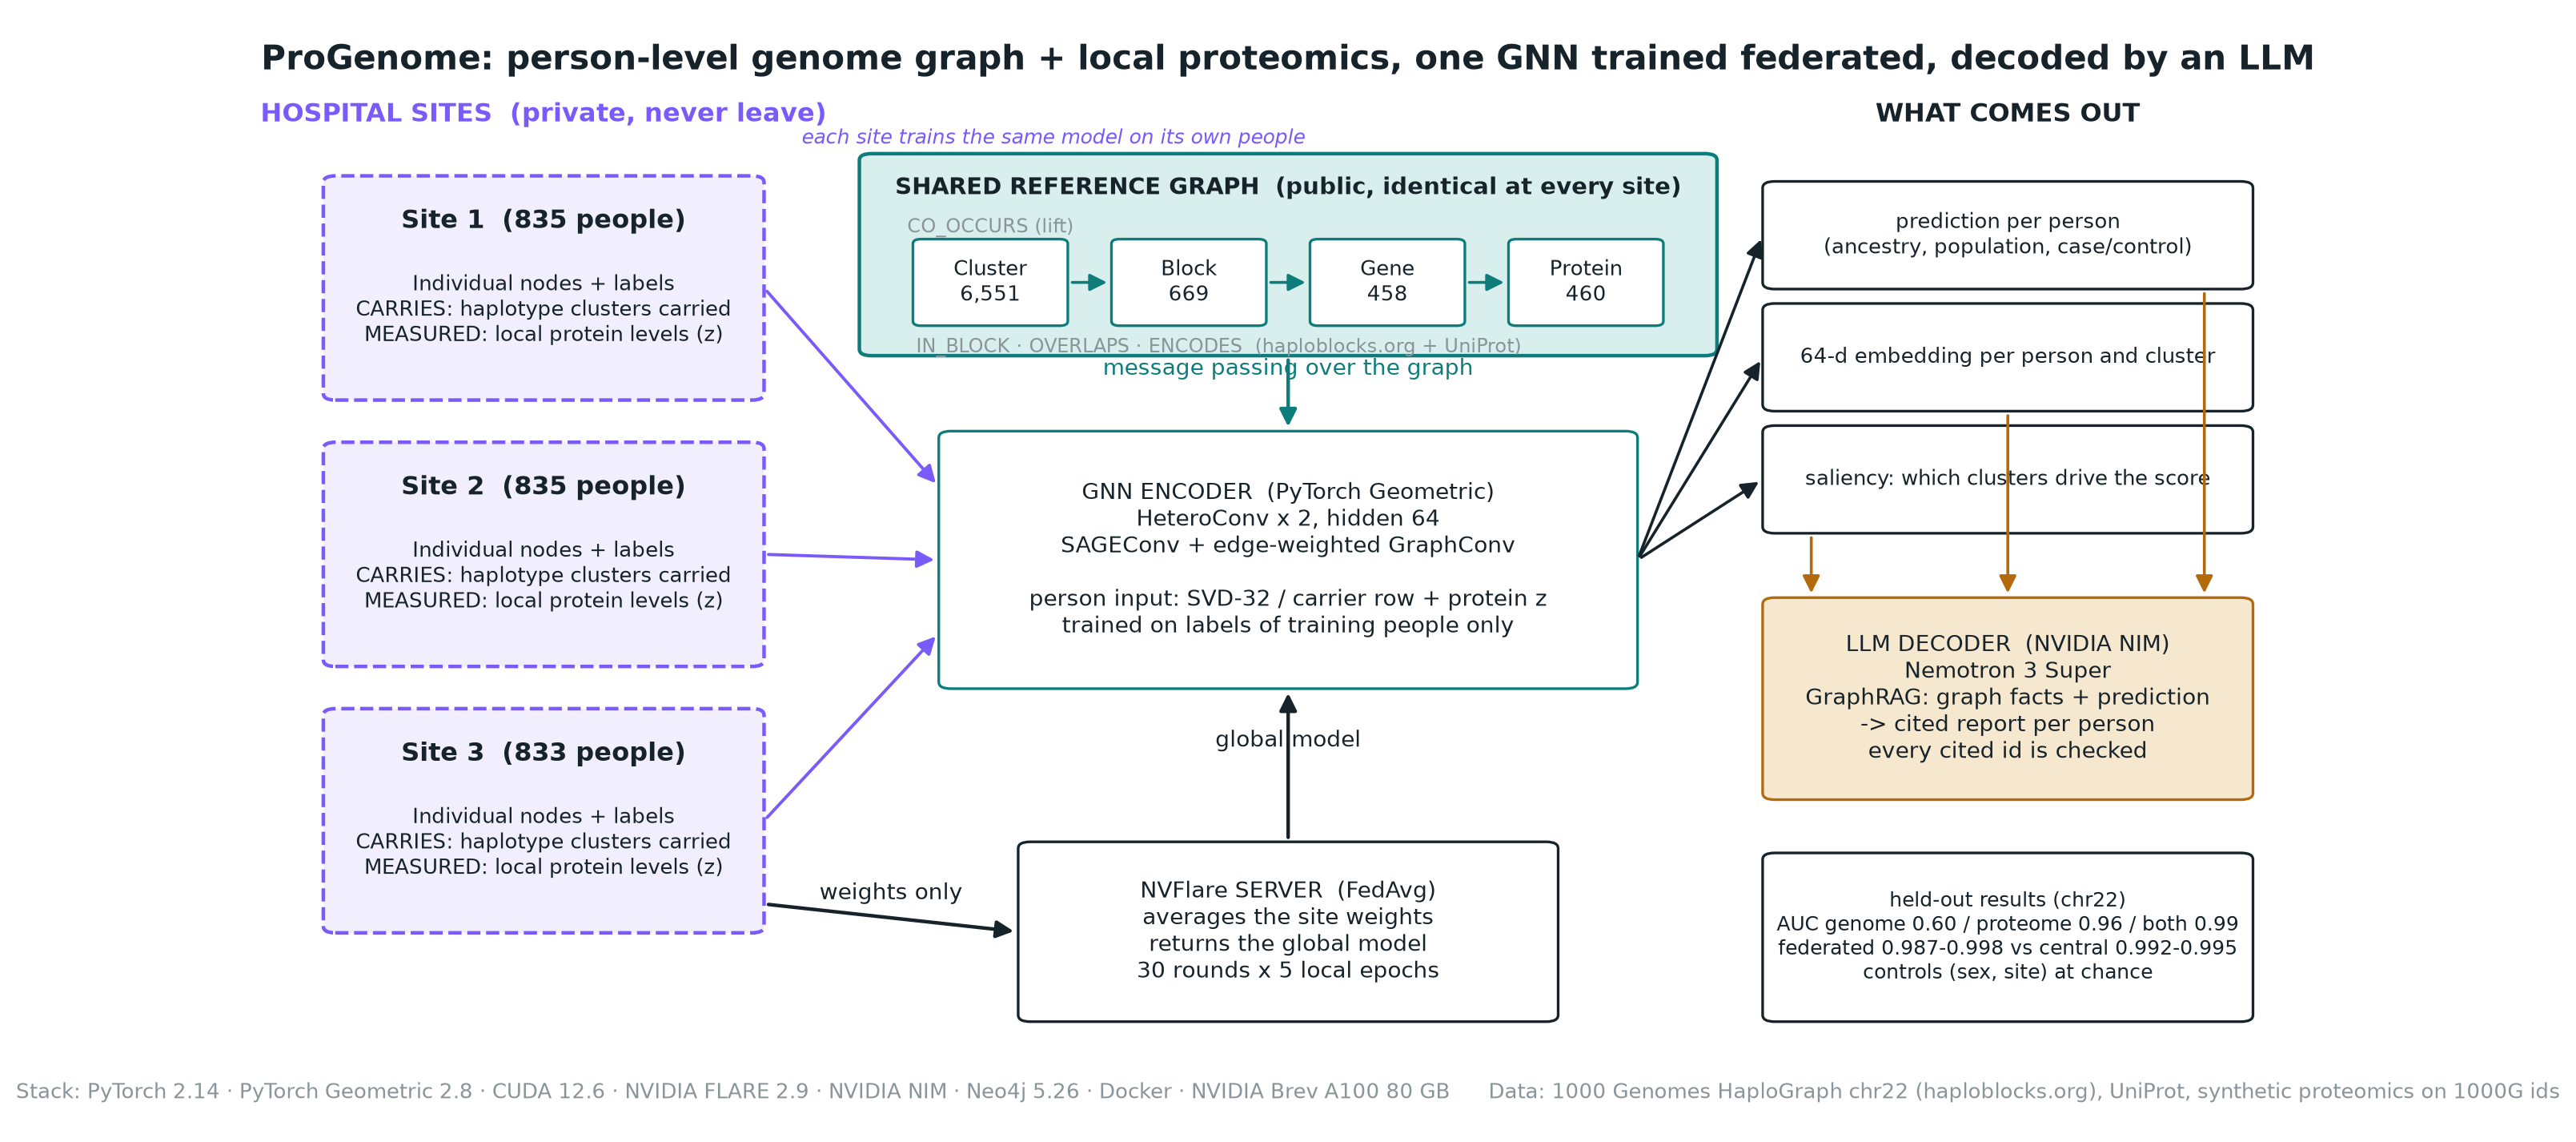
\includegraphics[width=0.98\linewidth]{architecture_slide.png}
\caption{System architecture on one page: private hospital sites, the shared reference graph, the GNN encoder trained through the NVFlare server, and the outputs feeding the LLM decoder.}
\end{figure}

\begin{longtable}{p{0.169\linewidth}p{0.442\linewidth}p{0.329\linewidth}}
\toprule
\textbf{Layer} & \textbf{Choice} & \textbf{Notes} \\
\midrule
\endhead
Language and data & Python 3.13, pandas 3.0, scipy 1.18 (sparse), scikit-learn 1.9 & pinned in requirements.txt \\
Graph learning & PyTorch 2.14, PyTorch Geometric 2.8, pyg-lib (random walks for Node2Vec) & torch\_cluster is deprecated in favour of pyg-lib; that caused the first image-build failure \\
Graph tooling & NetworkX 3.6, nx-cugraph (GPU dispatch), Neo4j 5.26 community in Docker & graph statistics, GraphML, browsing \\
Container & pytorch/pytorch:2.14.0-cuda12.6-cudnn9-runtime base, PIP\_BREAK\_SYSTEM\_PACKAGES=1, torch-tensorrt 2.14 & 10.5 GB image; runs on CPU when no GPU is present \\
Compute & Mac M2 CPU for development; NVIDIA Brev: L4 24 GB (GCP, \$0.85/h) and A100 80 GB (Crusoe, \$1.98/h) & brev\_deploy.sh creates or reuses an instance, uploads, builds natively, runs, copies outputs back \\
Inference & torch.compile (inductor): 36 ms $\rightarrow$ 4.9 ms per full graph, logits equal to within 0.0001 & Torch-TensorRT could not compile this scatter-heavy GNN within 3 hours and is not claimed \\
LLM & NVIDIA NIM, nvidia/nemotron-3-super-120b-a12b & key in the environment only; a local NIM container on the A100 would keep patient context on site \\
Federated & NVFlare 2.9 FedAvgRecipe, SimEnv simulator; federated/local\_only.py for the site-alone comparison & 3 clients as threads on one machine; POC mode across real machines is the next step \\
Packaging & Makefile (setup, run, run-v2, eda, decode, federated, docker, docker-run-v2, docker-federated, brev, report), setup.sh, run\_all.sh, run\_v2.sh, config.py + .env.example, 11 unit tests & clone-and-run on laptop or GPU; the image is the whole solution (data mounted, .env passed) \\
\bottomrule
\end{longtable}

Runtime, measured on 18 September from an empty folder (the verification runs of section 13):

\begin{longtable}{p{0.470\linewidth}p{0.235\linewidth}p{0.235\linewidth}}
\toprule
\textbf{Stage} & \textbf{Laptop, Apple M2 CPU} & \textbf{A100 80 GB (Docker)} \\
\midrule
\endhead
environment: venv or image, pinned dependencies, unit tests & 28 s (uv) & 3 min image build \\
v1: download, knowledge graph, statistics, baseline, plots, three GNN runs, embedding quality & 6 min & 3 min \\
v2: synthetic proteomics, graph v2, EDA, six GNN runs, ridge, decoder & 19 min & 4 min \\
federated: 30 rounds x 5 local epochs, central scoring, site-alone comparison & 4 min & 2 min \\
whole chain & about 30 min & about 14 min including the image build \\
one GNN training run & 30 s to 3 min & 1 to 16 s \\
one full-graph inference pass (2,548 people) & - & 36 ms eager, 4.9 ms compiled \\
one decoder call (NIM, remote) & 4 to 13 s & same \\
\bottomrule
\end{longtable}

\begin{figure}[htbp]
\centering
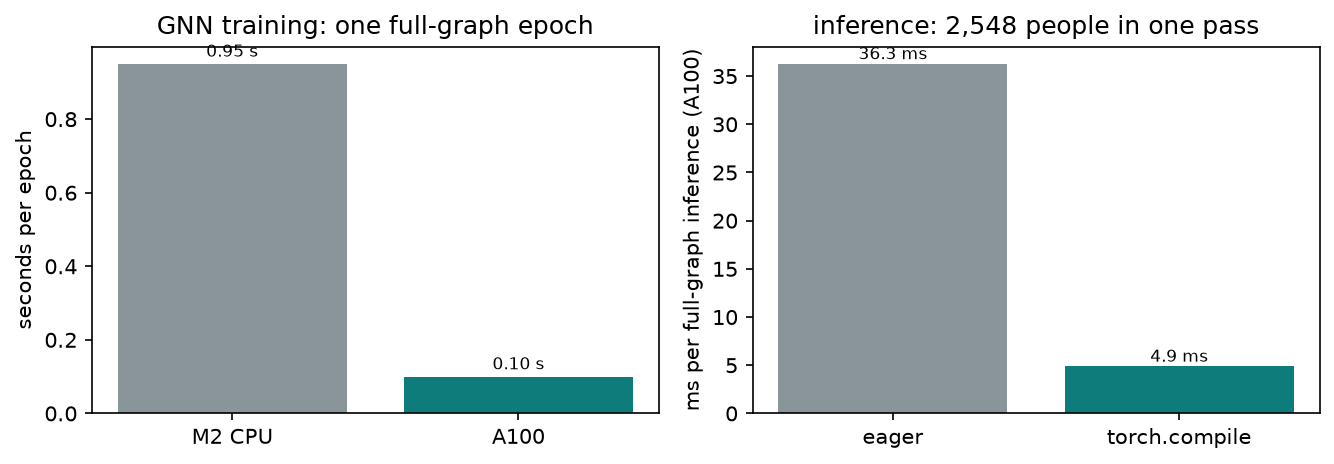
\includegraphics[width=0.85\linewidth]{compute_benchmarks.png}
\caption{Training epoch time on the laptop CPU versus the A100, and full-graph inference eager versus torch.compile on the A100.}
\end{figure}

\subsubsection{The Docker image, layer by layer}

The Dockerfile starts from pytorch/pytorch:2.14.0-cuda12.6-cudnn9-runtime (PyTorch with CUDA 12.6 already inside), sets PIP\_BREAK\_SYSTEM\_PACKAGES=1 because the base image's Python is system-managed, installs curl, copies requirements.txt and installs the pinned libraries, then tries three optional extras and prints a clear fallback message if any is unavailable for this torch build: pyg\_lib from the PyG wheel index (Node2Vec random walks; without it the code falls back to SVD), nx-cugraph from NVIDIA's index (NetworkX dispatches to cuGraph on the GPU; without it NetworkX runs on the CPU), and torch-tensorrt from the PyTorch cu126 index. It copies the code, runs the unit tests as part of the build so a broken image cannot be produced, and defaults to running run\_all.sh. Data and outputs are bind-mounted at run time, so the image never contains data. docker-compose.yml adds Neo4j 5.26 community with a persistent volume and the same pipeline image with GPU reservation.

\subsubsection{GPU deployment on Brev, step by step}

brev\_deploy.sh needs a logged-in brev CLI (brev login --api-key). It creates the instance if it does not exist (default an L4 on GCP; BREV\_INSTANCE=progenome-a100 selects the A100), waits until the instance reports RUNNING and READY, refreshes the SSH alias, checks nvidia-smi and docker over ssh, uploads genomics/ plus the two small proteomics inputs as one tarball, builds the image natively on the GPU box (no emulation, about 4 minutes on the A100), runs the whole v1 pipeline inside the container with the GPU, runs the inference benchmark (eager, torch.compile, TensorRT attempt) and copies outputs/ back to outputs\_brev/<instance>/. Billing continues until brev stop; the A100 is left running for the presentation.

\subsubsection{Inference and what torch.compile does}

infer.py rebuilds the exact inputs of a trained run, wraps the model so torch.compile sees plain tensors instead of dictionaries, times ten full-graph passes eager, then compiles with the inductor backend (kernel fusion and graph capture) or with the torch\_tensorrt backend and times again, and reports the maximum absolute logit difference so a speed-up cannot hide a numerical change. On the A100: 36.3 ms eager, 4.9 ms compiled (7.4x), maximum logit difference below 0.0001 across three runs, accuracy on all 2,503 labelled people 0.980 with SVD input. The TensorRT backend partitions the graph into dense parts it can compile (linear layers, norms) and scatter parts it cannot; on this hetero-GNN the compile step did not finish in three hours and is not part of any claim.

\subsection{13. How the goals were met, and what is not claimed}

\begin{longtable}{p{0.301\linewidth}p{0.470\linewidth}p{0.169\linewidth}}
\toprule
\textbf{Goal} & \textbf{Evidence} & \textbf{Status} \\
\midrule
\endhead
RQ1: one graph joining haploblocks, genes, proteins and people & schema v2 with 5 node types and 7 edge types, 2,548 people joined by id, browsable in Neo4j & done \\
RQ2: GNN combines genome and proteome & AUC 0.60 (genome) / 0.96 (proteome) / 0.99 (both); site control at chance; embedding silhouette 0.70; saliency finds causal clusters at 3x chance & done on synthetic ground truth \\
RQ3: federated training without moving records & NVFlare FedAvg over 3 sites, AUC 0.998 vs central 0.992 on the same people & done in simulation \\
Encoder $\rightarrow$ LLM decoder $\rightarrow$ insights & GraphRAG decoder with validated citations on Nemotron 3 Super & done \\
Reproducible and deployable & Makefile, Docker image, Brev deployment on L4 and A100, tests & done \\
\bottomrule
\end{longtable}

\begin{itemize}[leftmargin=1.4em]
  \item The case/control phenotype is synthetic: the integration numbers show the pipeline recovers a planted signal, not biology. Ancestry, population and sex results are on real labels.
  \item Chromosome 22 only; the code is chromosome-agnostic (CHROM=chr21 make run).
  \item On single-label accuracy the GNN ties, not beats, logistic regression; its value is the embedding space and the integration.
  \item The GNN embedding does not recover single-cluster cis effects; a per-protein ridge does for the strong ones.
  \item Federated evaluation reuses the central held-out people; a real deployment would report per site only.
  \item TensorRT is not part of the inference claim; torch.compile is.
\end{itemize}

\subsubsection{Verification and reproduction (18 September, before the commit)}

Before committing, the whole chain was re-run twice from the files that would be committed: once as a simulated fresh clone on the laptop (only the tracked files copied to an empty folder, then make setup, make run, make run-v2, make federated, make test) and once on the A100 with the Docker image rebuilt from the current Dockerfile, which had not been built since the pyg\_lib change. Both runs reproduce every count exactly and every model score within run-to-run noise (GPU kernels and FedAvg are not bit-reproducible). The rebuilt image contains pyg\_lib, so Node2Vec ran natively for the first time; with its original five pretraining epochs it was clearly undertrained (ancestry 0.80), with fifty epochs the loss converges and it becomes a working but slightly weaker alternative to SVD, so SVD remains the default everywhere and the deploy script now defaults to it. The decoder was also re-called on the laptop run; the language model's wording and the number of ids it chooses to cite vary between calls, the citation check is what stays constant.

\begin{longtable}{p{0.320\linewidth}p{0.207\linewidth}p{0.207\linewidth}p{0.207\linewidth}}
\toprule
\textbf{Quantity} & \textbf{Documented (original runs)} & \textbf{Fresh clone, laptop CPU} & \textbf{Rebuilt image, A100} \\
\midrule
\endhead
kept clusters / CARRIES / CO\_OCCURS & 6,551 / 2,365,574 / 187,030 & identical & identical \\
genes / proteins / MEASURED edges & 458 / 460 / 1,065,712 & identical & identical \\
ancestry-associated clusters (FDR 5\%) / sex & 6,470 / 0 & 6,470 / 0 & 6,470 / 0 \\
logistic baseline ancestry / population / sex & 0.977 / 0.614 / 0.463 & 0.977 / 0.614 / 0.463 & 0.981 / 0.614 / 0.463 \\
GNN v1 ancestry / population / sex (SVD input) & 0.974 / 0.437 / 0.503 & 0.974 / 0.437 / 0.503 & run with Node2Vec instead (next row) \\
GNN v1 with Node2Vec input, 50 epochs (A100 only) & not previously measured & - & 0.950 / 0.292 / 0.489 \\
embedding silhouette by ancestry: SVD / GNN & 0.06 / 0.70 & 0.06 / 0.70 & 0.06 / 0.70 (Node2Vec-initialised GNN) \\
phenotype AUC genome / proteome / both & 0.64 / 0.96 / 0.99 & 0.65 / 0.96 / 0.99 & 0.64 / 0.96 / 0.99 \\
site control balanced accuracy (chance 0.33) & 0.30 & 0.34 & 0.30 \\
saliency: causal clusters in top 20 & 4 & 4 & 4 \\
ridge: cis proteins with R2 > 0.1 / others & 4 / 0 & 4 / 0 & 4 / 0 \\
federated 30 rounds AUC / central AUC, same 376 people & 0.998 / 0.992 & 0.996 / 0.994 & 0.987 / 0.995 \\
site-alone AUC on own test people vs federated model on the same people & not previously measured & - & 0.998 / 0.986 / 0.988 vs 0.999 / 1.000 / 0.968 \\
decoder: cited ids / invented ids & 25 / 0 & 4 / 0 (4.2 s) & dry run (no key on the box) \\
inference eager / torch.compile (A100) & 36 ms / 4.9 ms & - & 36.3 ms / 4.9 ms (7.45x, max logit diff 1.9e-06) \\
unit tests & 11 pass & 11 pass (make setup) & 11 pass (docker build) \\
\bottomrule
\end{longtable}

\subsection{14. Team context}

Friederike Duendar (lead) wrote the README's research questions, the UniProt gene BED and an R exploration of gene-block overlaps; Nolan Bruyat built the synthetic proteomics generator and its plots; Zillur Rahman built the proteomics-side analysis now on main (see below); Yan Zhou coordinates the manuscript (two introduction paragraphs, two methods paragraphs, one results paragraph); Anita Egebor and Alvaro Martinez Barrio contributed to the README and data access. The genomics/ pipeline described here is the modelling backbone into which those pieces plug.

\subsubsection{What is on main since this branch was created, and how it relates}

The team's proteomics work on main (the synthetic proteomics generator with 4,000 SITE-id samples, protein filtering and classification baselines, a protein-centred knowledge graph built from the HaploGraph edge list annotated with UniProt proteins, a federated comparison of feature sets, and methods\_and\_results.md) covers the proteome side and the federated logistic setting. genomics/ adds the genome side: the person-level knowledge graph on the 1000 Genomes ids, the graph neural network, the LLM decoder and the NVFlare run. The two share the same HaploGraph edge file, the same UniProt gene BED and the same three-site design, and they are complementary: nothing in genomics/ touches a path on main, so the branch merges cleanly, and for the manuscript the proteomics analysis and the graph model plug into the same methods and results structure.

\section{Part IV: Reference}

\subsection{Run it yourself}

From a fresh clone of the repository on branch modelling, on a laptop or a GPU machine:

\begin{small}\begin{verbatim}
git clone https://github.com/collaborativebioinformatics/ProGenome.git
cd ProGenome && git checkout modelling && cd genomics
make setup          # .venv with torch (CPU, or CUDA if nvidia-smi works), pinned deps, unit tests
make run            # v1: download -> graph -> statistics -> baseline -> plots -> GNN (ancestry, population, sex) -> embeddings
make run-v2         # v2: synthetic proteomics -> graph v2 -> EDA -> GNN ablations -> ridge -> decoder dry run
make federated ROUNDS=30 LOCAL_EPOCHS=5     # NVFlare FedAvg over 3 sites, then central scoring
make neo4j-load     # browse the graph at http://localhost:7474  (neo4j / progenome)
make docker && make docker-run              # the same v1 chain inside the CUDA image
BREV_INSTANCE=progenome-a100 make brev      # build and run on the A100, copy outputs back
make decode WHO=HG00103                     # LLM insight for one person (needs NVIDIA_API_KEY)
make test           # 11 unit tests on a toy graph
make help           # every target
\end{verbatim}\end{small}

Single stages take a --chrom flag and, where relevant, --target, --modality, --init; for example .venv/bin/python train\_gnn\_v2.py --target phenotype --modality both --init raw reproduces the combined model with saliency, and .venv/bin/python infer.py --run ancestry\_svd --compile inductor reproduces the inference benchmark. Every output path is relative to genomics/, and data/, outputs/ and outputs\_brev/ are git-ignored.

\subsection{Secrets and configuration}

Configuration enters the code in one place, config.py, which reads genomics/.env, then \textasciitilde{}/.progenome.env, then defaults, with exported shell variables taking precedence; .env.example lists every variable with a comment (NVIDIA\_API\_KEY, NIM\_MODEL, NIM\_URL, NEO4J\_URI/USER/PASSWORD, HAPLOBLOCKS\_BASE, CHROM, data and output directories, BREV\_INSTANCE/TYPE) and make config prints what is in effect with secrets masked. The shell scripts source the same files through load\_env.sh, and the Docker targets pass .env into the container. The only secret is the NVIDIA API key; .env is git-ignored, nothing under the repository contains a key, and the decoder refuses to call the endpoint without one instead of falling back silently. Versions are pinned in requirements.txt (torch 2.14.0, torch\_geometric 2.8.0.post1, pandas 3.0.5, scipy 1.18.1, scikit-learn 1.9.1, networkx 3.6.1, neo4j 6.3.1, nvflare 2.9.0, pytest 9.1.1) and setup.sh installs torch from the CPU or cu126 index depending on whether a GPU is present.

\subsection{Repository map (genomics/)}

\begin{small}\begin{verbatim}
haplokg.py, build_kg.py            knowledge graph v1 (people, clusters, blocks)
haplokg_proteins.py, build_kg_v2.py  genes, proteins, harmonised measurements (v2)
proteomics_synth_1000g.py            synthetic proteomics on 1000G ids with ground truth
cooccurrence_analysis.py, eda.py     statistics and the EDA report
baseline.py                          logistic regression + the shared split
graph_explore.py, neo4j_load.py      NetworkX statistics/plots, Neo4j loader
train_gnn.py, train_gnn_v2.py        the GNN (genome; genome+proteome)
embeddings.py                        embedding quality and plots
proteome_linear_baseline.py          per-protein ridge (genome -> proteome)
graphrag_decoder.py                  NIM LLM decoder
infer.py                             inference benchmark
federated/{model,client,job,evaluate_global}.py   NVFlare FedAvg
Dockerfile, docker-compose.yml, Makefile, setup.sh, run_all.sh, run_v2.sh, brev_deploy.sh
docs/architecture.html (.mmd), METHODS.md, DEEP_DIVE.md, report/
tests/                               unit tests on a toy graph
\end{verbatim}\end{small}

\subsection{Glossary}

\begin{longtable}{p{0.235\linewidth}p{0.705\linewidth}}
\toprule
\textbf{Term} & \textbf{Meaning} \\
\midrule
\endhead
Haploblock & a stretch of chromosome between recombination hotspots, inherited as a unit \\
Haplotype & one copy's sequence of a block; each person has two per block \\
Cluster & a group of near-identical haplotypes of one block (MMseqs2); a person carries it if either haplotype is in it \\
Carrier matrix & people x clusters 0/1 matrix; the CARRIES edges \\
Lift & how much more often two clusters co-occur than chance: P(A and B) / (P(A) P(B)) \\
Cramer's V & effect size of a contingency test, 0 (independent) to 1 (perfectly associated) \\
FDR & false discovery rate; Benjamini-Hochberg controls the expected fraction of false positives among findings \\
SVD & singular value decomposition; here a 32-component factorisation of the carrier matrix giving embeddings \\
GNN / message passing & neural network on a graph; each layer mixes a node's vector with its neighbours' \\
SAGEConv / GraphConv & two PyG layer types: neighbour-mean aggregation; edge-weighted aggregation \\
Balanced accuracy / AUC & mean per-class recall; probability a random case outscores a random control \\
Harmoniser & per-site, per-protein robust z-score removing batch offsets \\
MNAR & missing not at random; here low-abundance proteins go missing first \\
FedAvg & federated averaging of model weights across sites \\
NIM & NVIDIA Inference Microservice; an OpenAI-compatible LLM endpoint \\
Brev & NVIDIA's GPU cloud; instances by the hour \\
\bottomrule
\end{longtable}

\end{document}
